%------------------------------------------------------------------------------
%
%  Documentation "Data Logging Service"
%
%  Ingenieurgemeinschaft IgH
%
%  Author: Florian Pose
%
%  vim: spelllang=en spell tw=78
%
%  Permission is granted to copy, distribute and/or modify this document under
%  the terms of the GNU Free Documentation License, Version 1.3 or any later
%  version published by the Free Software Foundation; with no Invariant
%  Sections, no Front-Cover Texts and no Back-Cover Texts. A copy of the
%  license is included in the file fdl-1.3.txt.
%
%------------------------------------------------------------------------------

\documentclass[a4paper,12pt,BCOR6mm,bibtotoc,idxtotoc]{scrbook}

\usepackage[english]{babel}
\usepackage[utf8]{inputenc}
\usepackage{graphicx}
\usepackage[automark,headsepline]{scrpage2}
\usepackage{makeidx}
\usepackage{listings}
\usepackage{hyperref}

\lstset{basicstyle=\ttfamily\small}
\lstset{numberstyle=\tiny}
\lstset{aboveskip=4mm}
\lstset{belowskip=2mm}
\lstset{escapechar=`}

\hypersetup{pdfpagelabels}
\hypersetup{plainpages=false}
\hypersetup{linkcolor=blue}
\hypersetup{urlcolor=blue}
\hypersetup{colorlinks=true}

\setlength{\parskip}{1.5ex plus 0.8ex minus 0.5ex} \setlength{\parindent}{0mm}

\newcommand{\IgH}{\raisebox{-0.7667ex}\
    {
\includegraphics[height=2.2ex]{bilder/ighsign}}}

\DeclareFontShape{OT1}{cmtt}{bx}{n} {
<5><6><7><8><9><10><10.95><12><14.4><17.28><20.74><24.88>cmttb10 }{}

\def\revision{8484e7aef7bb}
\def\isodate#1-#2-#3 #4:#5 #6x{
  \day  = #3
  \month= #2
  \year = #1
}
\isodate 2019-09-04 12:46 +0000x


\makeindex

\begin{document}

%------------------------------------------------------------------------------

% Titelseite

\pagenumbering{roman} \pagestyle{empty}

\begin{titlepage} \begin{center} \rule{\textwidth}{1.5mm}

{\Huge\bf Data Logging Service (DLS)\\[1ex] Version 1.2}

\vspace{1ex}

\rule{\textwidth}{1.5mm}

\vspace{\fill}

{\Large Florian Pose, \url{fp@igh-essen.com}\\[1ex]
    Ingenieurgemeinschaft \IgH}

\vspace{\fill}

The ``DLS'' is a data logging system capable of collecting high-frequency data
over a long period and storing them in a highly compressed fashion. Its
objective is to grant the user unrestricted, high-performance access to the
acquired data at all times: whether the overview for a whole year or just a
tiny variation in a fraction of a second is needed.

\vspace{\fill}

{\large Essen, \today\\[1ex] Revision \revision}

\end{center}
\end{titlepage}

%------------------------------------------------------------------------------

% Inhaltsverzeichnis

\pagestyle{scrheadings}

\tableofcontents

%------------------------------------------------------------------------------

% Dokument

\chapter{General}
\label{sec:allg}
\pagenumbering{arabic}

%------------------------------------------------------------------------------

\section{Principles of data acquisition}
\label{sec:allg_grund}

The ``Data Logging Service'' (hereinafter \textit{DLS})\index{DLS} is
a data logging system that is not only able to collect, compress and store any
type of measured data over a long period, but also to display them quickly
whenever required.

Prerequisite for a data logging process is a \textit{data source}\index{data
source!Definition}, which provides the measured data. In this case it is a
server that provides the measured data of the \textit{rt\_lib}, developed by
the \textit{IgH}, via the network. The communication with the data source is
described in \autoref{sec:dlsd_logger_comm}.

All data to be delivered are organised in
\textit{channels}\index{channel!definition}. A channel is the abstraction of a
measurable physical quantity provided by the data source. The properties of a
channel are the unit\index{channel!unit}, the maximum sampling
frequency\index{channel!sampling frequency} and the data
type\index{channel!data type}.

The DLS can connect to the data source and thus interrogate the information
via the provided channels. In the same way it is then capable of requesting
and receiving the measured data for specific channels.

%------------------------------------------------------------------------------

\section{Measurement jobs}
\label{sec:allg_jobs}

The DLS acquires data by means of so-called \textit{measurement
jobs}\index{measurement job!definition}. They comprise general specifications
for data acquisition along with the list of the channels to be included and
their specifications. A measurement job is always bound to a certain data
source. It is possible that any number of measurement jobs is available at the
same time.

Data from different channels can simultaneously be acquired within the scope
of one measurement job. For this purpose, every channel to be included must be
provided with a so-called \textit{channel specification}\index{channel
specification}. This summarises the conditions, under which data from a
certain channel are to be acquired and stored. It includes the sampling
frequency, the block size, the meta data to be acquired (see
\autoref{sec:dlsd_data_meta}), the meta reduction ratio and the compression
method.

%------------------------------------------------------------------------------

\section{Data storage}
\label{sec:allg_ablage}

The acquired data are stored in the DLS data directory\index{DLS data
directory} together with the acquisition specifications, time and channel
information and sorted according to measurement jobs. This is the current
directory by default. If another storage location is desired, this fact can be
communicated to the programs of the DLS package either via the command line
parameters (option \texttt{-d}) or stored in the environment variable
\$DLS\_DIR\index{\$DLS\_DIR}. The search order is always: Parameter --
environment variable -- current directory.

It is certainly possible that several DLS data directories exist at a time,
which, however, must be served by different instances of the DLS daemon (see
\autoref{sec:dlsd_mother}).

A detailed description of the DLS data directory’s structure and the data
contained therein can be found in \autoref{sec:data}.

%----------------------------------------------------------------------------

\section{Tools}
\label{sec:allg_tools}
\index{tools}

\begin{description}

\item[DLS Manager]\index{DLS Manager} Measurement jobs\index{measurement job}
can be edited by means of a graphical user interface, the \textit{DLS Manager}
(see \autoref{sec:manager}). It allows the user to create new measurement jobs
and adapt existing ones. This can be done during a data acquisition. The user
can also see whether data acquisition is currently being performed.

\item[DLS View] A graphical tool \textit{DLS View}\index{DLS View} is provided
to view the data (see \autoref{sec:view}). The user can have any of the
channels involved in a measurement job be displayed above a common time scale.
Here, it is also possible to navigate in the time window and to determine
individual data values.

\item[dls] The command line tool \textit{dls}\index{dls (tool)} recognises
commands to view and export data that have already been acquired. See
\autoref{sec:apx_cmd_dls} for a list.

\item[Init-Script]\index{Init Script} An init script is provided for starting
and stopping the dlsd and all associated services. It recognises the
parameters \texttt{start}, \texttt{stop}, \texttt{restart} and
\texttt{status}. The configuration of the service is made via a sysconfig
file\index{sysconfig file} which contains all required variables. It is
recommended to export the included variables via the profile script, which is
provided as well, and to thus make them accessible to all users.

\item[dls\_status] The Script \textit{dls\_\-status}\index{dls\_status} serves
for the general monitoring of the data acquisition. It is a command line tool
that can display the basic readiness for data logging for a certain DLS data
directory. It displays whether the DLS parent process is running, which
measurement jobs are available and whether for these jobs the corresponding
DLS acquisition processes are running.

\end{description}

%------------------------------------------------------------------------------

\chapter{The DLS daemon (dlsd)} \label{sec:dlsd}

The \textit{DLS daemon} (short: \textit{dlsd}) serves for the entire data
acquisition and data storage\index{dlsd}. It is a process that is running in
the background (without being connected to a console) and is bound to a
specific DLS data directory\index{DLS data directory}. It must always be
running when data are to be acquired.

A representation of the entire system architecture\index{architecture} can be
seen in \autoref{fig:arch}.

\begin{figure}[htb] \begin{center} 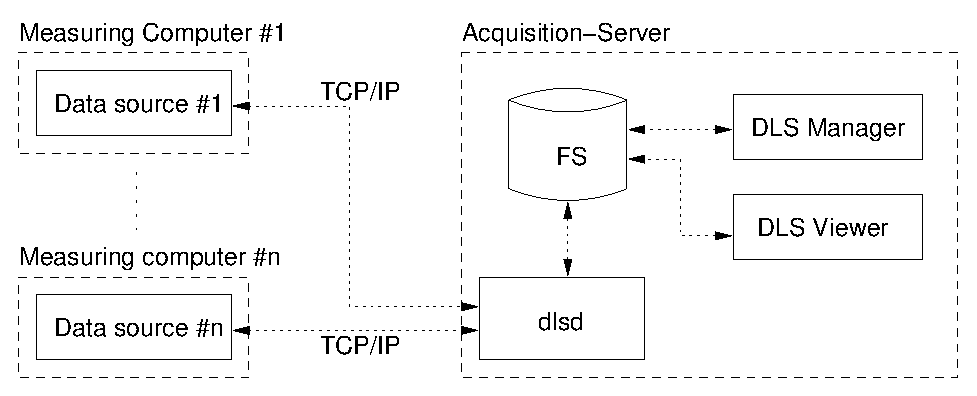
\includegraphics[width=250pt]{bilder/arch_en} \end{center} \caption{Architecture} \label{fig:arch} \end{figure}

%------------------------------------------------------------------------------

\section{The dlsd parent process}
\label{sec:dlsd_mother}
\index{dlsd!parent process}

A dlsd process started by the user or system will monitor the measurement
jobs\index{measurement job}. It is then called \textit{dlsd parent process}.
In the memory it holds available a list of dedicated copies of the job
specifications existing in the DLS data directory, which additionally contain
information on the associated acquisition processes.

Every started parent process must work in a different DLS data
directory\index{DLS data directory}. This is ensured by implemented protective
mechanisms (\textit{PID files}\index{PID files}, see \autoref{sec:apx_pid}).

%------------------------------------------------------------------------------

\subsection{Behaviour of the dlsd parent process}
\label{sec:dlsd_mother_behaviour}

Initially, the parent process reads in all measurement job specifications in
the DLS data directory and fork a child for every active
measurement job \index{measurement job} (\textit{dlsd acquisition process}, see
\autoref{sec:dlsd_logger}), which will thereafter serve for the data
acquisition of the measurement job concerned. Subsequently, it performs the
following tasks in a defined time interval:

\begin{itemize}

\item Check whether signals have been received in the meantime. That can
happen, for instance, when the dlsd is to be terminated or when one of the
acquisition processes was terminated (see \autoref{sec:dlsd_mother_signals}).

\item Check the spooling directory for new entries. If in the spooling
directory one or more files are found, they are assessed as spooling
information and processed as described in \autoref{sec:dlsd_mother_spooling}.

\item Check of the acquisition processes. The parent process shall ensure that
for every active measurement job there will always run a corresponding
acquisition process.

\end{itemize}

%------------------------------------------------------------------------------

\subsection{Spooling} \label{sec:dlsd_mother_spooling} \index{Spooling}

A spooling process helps to ensure a smooth operational sequence when measurement jobs \index{measurement job} are changed during data acquisition. Since the measurement jobs are organised in files, without such a process the requirement that a specifications file is not simultaneously read by the dlsd while the user is writing would not safely be met. This might result in processing errors.

Therefore, the DLS data directory contains a subdirectory \texttt{spool}. The dlsd parent process empties this directory when starting and will then, once only, enter all job specifications. Thereafter, it will access the job specifications for reading them only when accordingly and explicitly requested by a spooling command.

For the dlsd, a valid spooling command is a file with any name in the spooling directory, which contains only an ASCII-coded job ID (positive integer). This ID enables the dlsd to decide what to do:

\begin{itemize}

\item If it does not yet know a job with this ID, it will assume that the job
has been newly created. It will import it and start the corresponding
acquisition process, if required.

\item If, however, it knows a job with this ID \textbf{and} the file with the
job specifications exists (\textit{job.xml} see chapter
\autoref{sec:data_jobs}), the specifications will be newly read in and the
acquisition process will be started, stopped or notified, as appropriate.

\item If it knows a job with this ID but the specifications file does
\textbf{not} exist, the dlsd will assume that the job was deleted. It will
terminate a possibly running acquisition process and cancel the specification
from its list.

\end{itemize}


Generally, the spooling file is deleted to confirm that the new information has been received. If an error occurs during processing, the file will be left in the spooling directory.

%------------------------------------------------------------------------------

\subsection{Signal processing} \label{sec:dlsd_mother_signals} \index{signal processing}

The following signals are processed by the dlsd parent process:

\begin{description}
\item[SIGCHLD] A child process was terminated. This may have different reasons: \begin{itemize}
\item The process was explicitly terminated and has the return value 0 (no error). In that case it will be restarted with the next check, because the process was not terminated according to the specifications and the data acquisition must be continued as soon as possible.
\item The process has detected an internal error and has terminated itself with the return value $-1$. This will be recognised accordingly by the parent process so that the process will not be restarted. The user, however, will not receive an explicit warning that the data acquisition has stopped running. A message will only be sent to the \textit{syslogd}\index{syslogd}.
\item The process had a timing error and has terminated itself with the return  value $-2$. The process will be restarted by the parent process after a defined time span has elapsed. \end{itemize}
\item[SIGINT/SIGTERM] The dlsd is to be terminated. The parent process will forward the signal to all of its child processes, wait until they have stored their data and then terminate itself with the return value 0 (no error).
\item[SIGSEGV and others] These signals are monitored for safety and treated alike by the dlsd parent process and acquisition process. When such a state occurs, the process will leave a file with the name \textit{error\_\textless PID\textgreater} in the DLS data directory which contains information about the signal received and shortly thereafter terminate itself with the return value $-3$. \end{description}

%------------------------------------------------------------------------------

\section{The dlsd acquisition process}
\label{sec:dlsd_logger}
\index{dlsd!acquisition process}

The acquisition process that was split off the dlsd parent process serves for
the communication with the data source, the compressing of the received data
and the storing of the compressed data on the hard disk. It is associated with
a specific measurement job\index{measurement job} that was assigned to it by
the dlsd parent process at the start. This measurement job is uniquely
identified via the DLS data directory and the corresponding measurement job
ID. All data referring to this job are stored there in the subdirectory
\textit{job\textless ID\textgreater} (see \autoref{sec:data}).

%------------------------------------------------------------------------------

\subsection{Behaviour of the acquisition process} \label{sec:dlsd_logger_behaviour}

The dlsd acquisition process will first import the specifications of its
measurement job\index{measurement job} from the central specifications file
\textit{job\textless ID\textgreater/job.xml} and then connect via TCP/IP with
the data source indicated there (description of the communication protocol,
see \autoref{sec:dlsd_logger_comm}).

For every channel the acquired measured data go to a so-called \textit{block buffer}. When this is full, the data will be block-wise compressed, stored and indicated with the time stamp of the first data value in the block. The advantage of this approach is that the compression does not require a streaming process and the individual data values will be clearly identifiable later on. The size of this data block\index{data block} (and thus of the \textit{block buffer}) can be defined by the user in the channel specifications.

In this connection, a sequence of data blocks that is continuous in terms of
time is designated as \textit{chunk}\index{chunk!Definition}. This contains
those measured data of an individual channel that have been acquired in a
continuous, completed time domain. It combines the underlying channel
specification with the real properties of the respective channel of the data
source and the ultimately acquired data (see \autoref{sec:data_chunks}).

%------------------------------------------------------------------------------

\subsection{Generation of meta data} \label{sec:dlsd_data_meta}

In order to provide a fast preview even with large amounts of data, the DLS acquisition process does not only store the (``generic'') data values\index{data!generic} that were received from the data source but additionally saves data that have been aggregated over certain time spans, so-called ``meta data''\index{meta data}. The latter exist in various reduction levels, the so-called ``meta levels''. A read process can then - according to the desired resolution - decide, which meta level it is going to use and thus load the data very quickly.

Mathematically, this means that the complexity of the algorithm for the
loading of $n$ data values of a time span $\Delta t$ and a sampling frequency
$f$, where: $n = \Delta t \cdot f$ no longer is $O(n)$, i.\,e. linear
dependent on the number of underlying data values in the period, but remains
dependent only on the number of supporting points desired in the current
resolution, which again is independent of the number of underlying data
values. Accordingly, in terms of time and storage requirement, the algorithm
is of order $O(1)$.

To generate the (redundant) meta data, in the dlsd acquisition process a
so-called \textit{meta buffer} is provided in parallel with the block buffer.
This buffer has a capacity for $u$ data values with $u$ being the so-called
meta reduction ratio\index{meta reduction ratio}, which the user can define in
the channel specifications. The meta reduction ratio applies for all levels.
When the meta buffer is full, from the $u$ generic data values a ``meta data
value'' of meta level 1 will be generated and stored there in a block and a
meta buffer. For these buffers again the same rules apply as for the level of
the generic data, i.\,e. the meta levels are generated in ``cascaded'' fashion.
Accordingly, storage space for a new level will be reserved only when the
first meta value of this level is provided.

There are different types of meta data\index{meta types}, which can also be
generated simultaneously.  At present the following types are supported:

\begin{description}

\item[Mean values] (``mean'', mask bit 0) A meta value of level $n$ is the
arithmetic means value of $u$ values of level $n - 1$.

\item[Minima] (``min'', mask bit 1) A meta value of level$n$ is the smallest
of $u$ values of level $n - 1$.

\item[Maxima] (``max'', mask bit 2) A meta value of level $n$ is the largest
of $u$ values of level $n - 1$.

\end{description}

Which types of meta values are ultimately to be generated during the data
acquisition, can be determined by the user in the channel specifications with
the so-called meta mask\index{meta mask}. This is produced by the bit-wise
\textit{OR} operation of the indicated mask bits. (Examples: ``Mean values,
minima and maxima'' corresponds to meta mask 7, ``only mean values''
corresponds to meta mask 1, and ``minima and maxima'' corresponds to meta mask
6).

It is almost always the case that when completing a chunk\index{chunk} less
than $u$ values remain on a level. From these values \textbf{no} further meta
value will be generated since when being displayed this data value would in
all likelihood be narrower than one pixel. The values remaining in the meta
buffers will consequently be discarded.

%------------------------------------------------------------------------------

\subsection{Communication with the data source}
\label{sec:dlsd_logger_comm}

The communication with the data source is effected via the protocol for the
\textit{rt\_lib} (version \textit{$\ge 2.7$}) from \textit{IgH} based on
XML\index{XML}. The connection to the data source is established via TCP/IP
(port 2345).

\paragraph{Identification of the data source} After the connection has been
established, first a \textit{\textless connected\textgreater}-Tag is awaited,
which as \textit{name} attribute must contain the value \textit{MSR} (German
\glqq Messen -- Steuern -- Regeln\grqq, which means ``instrumentation and
control''). The coded version of the data source software in the
\textit{version} attribute is checked for compatibility with the current dlsd
version. Additionally, the \textit{\textless connected\textgreater}-Tag may
contain an \textit{arch} attribute, which contains the architecture
(``endianness''\index{endianness}) of the data source and thus of the binary
data sent. Potential values are \textit{big} (for ``big endian'') or
\textit{little} (for ``little endian''). If no \textit{arch} attribute exists,
the source architecture is assumed to be ``little endian'' and a warning is
issued.

\paragraph{Determination of the maximum sampling frequency} When the
\textit{\textless connected\textgreater}-Tag sent from the data source has
been received and verified, the acquisition process will first query the MSR
parameter \textit{/Taskinfo/Abtastrate} (sampling frequency) and then wait for
the answer. This value (the maximum sampling frequency of the data source)
will later be needed for checking the plausibility of the channel
specifications and for calculating the reduction ratio of the sampling
frequencies.

\paragraph{Readout of all channels} Subsequently, the complete list of the
channels provided by the data source will be requested with an
\textit{\textless rk\textgreater} command. The response of the data source
must begin with an introductory \textit{\textless channels\textgreater}-Tag,
which is followed by the individual channels, which are described in a
\textit{\textless channel\textgreater}-Tag each. The end of the channel list
is again marked with a \textit{\textless /channels \textgreater}-Tag.

Example of a response of the data source to an \textit{\textless rk
\textgreater} command:

\begin{lstlisting}[basicstyle=\ttfamily\scriptsize]
<channels>
 <channel name="/Time" unit="s" alias="" index="0" `$\hookleftarrow$`
  typ="TDBL" bufsize="50000" HZ="10000" value="1112814601.3209"/>
 <channel name="/Taskinfo/Controller_Execution_Time" unit="us" `$\hookleftarrow$`
  alias="" index="6" typ="TUINT" bufsize="50000" HZ="10000" value="22"/>
 <channel name="/Taskinfo/Controller_Call_Time" unit="us" alias="" `$\hookleftarrow$`
  index="7" typ="TUINT" bufsize="50000" HZ="10000" value="99"/>
 <channel name="/Istwert/Kraft" unit="N" alias="" index="9" `$\hookleftarrow$`
   typ="TDBL" bufsize="50000" HZ="10000" value="-0.6745"/>
 <channel name="/Istwert/Druck" unit="bar" alias="" index="12" `$\hookleftarrow$`
  typ="TDBL" bufsize="50000" HZ="10000" value="0.1372"/>
</channels>
\end{lstlisting}

Of the attributes in the \textit{\textless channel\textgreater}-Tag the
following will be saved for later use:

\begin{description}

\item[name] -- Channel name (unique)

\item[unit] -- Unit of the channel (is stored as a string, optional)

\item[index] -- The position of the channel within the list. This will later
also be used as an identifier for a channel directory within the DLS data
directory (see \autoref{sec:data}).

\item[typ] -- Data type. This must be one of the known data types from the
table in \autoref{sec:apx_types}, in order to enable the processing of any
data received later on.

\item[bufsize] -- Size of the circular buffer within the data source. This
will later be used for checking the plausibility of a given sampling
frequency:

$ \hbox{BlockSize} \cdot \hbox{Reduction} \stackrel{!}{\le} \frac{\hbox{BufferSize}}{2} $

\item[HZ] - Channel-specific, maximum sampling frequency.

\end{description}

All of these channel information details are filed in a list in the memory of
each acquisition process and will be used for the plausibility checks whenever
adding or changing a channel specification.

\paragraph{Start of data acquisition} When the acquisition process recognises
the channels list, the data acquisition will be started (unless it is required
that previously the trigger parameter is waited for). This is done via the
\textit{\textless xsad\textgreater} command, which is sent once for each
channel to be acquired. Attributes of the command are:

\begin{description}

\item[channels] - Contains the index of the queried channel in the list of all
channels,

\item[reduction] - the (integer) scaling-down factor of the maximum sampling
frequency of the channel to describe the absolute sampling frequency,

\item[blocksize] - the number of values to be sent in a block (this value
being completely independent of the block size in the channel specification),
and

\item[coding] - the coding of the data that is currently defined on
\textit{Base64}.

\end{description}

A typical command for starting the data acquisition of a channel could
therefore look as follows:

\begin{lstlisting}[basicstyle=\ttfamily\scriptsize]
<xsad channels="7" reduction="100" blocksize="1000" coding="Base64"/>
\end{lstlisting}

\paragraph{Receipt of data} The acquisition process now waits for a
\textit{\textless data\textgreater} tag that is the beginning of a block of
channel data tags. This tag must contain a \textit{time} attribute
corresponding to the time stamp of all last data values each in the following
channel data tags. These are expected to be \textit{\textless
F\textgreater}-Tags, which contain the last measured data of a single channel
each and have the attributes \textit{c} (channel index) and \textit{d} (coded
measured data). The last \textit{\textless F\textgreater}-Tag must be followed
by a \textit{\textless /data\textgreater}-Tag  tag that will return the
acquisition process to the waiting state.

\paragraph{Change of channel specifications} If a channel specification is
changed during data acquisition, the acquisition process will send another
\textit{\textless xsad\textgreater}-Tag, which in addition to the new channel
specifications contains an \textit{id} attribute representing a
(connection-wide) unequivocal command identifier. If the data source has
accepted the channel specifications and if the next data of the channel
involved definitively comply with the \textbf{new} specifications, the data
source is expected to send an \textit{\textless ack\textgreater}-Tag  tag
beforehand, the attribute of which is the command ID of the respective
\textit{\textless xsad\textgreater}-Tags. The acquisition process, too, will
then finally be changed to comply with the new channel specifications.

%------------------------------------------------------------------------------

\subsection{Limitation of the data volume (quota)}
\label{sec:dlsd_logger_quota}
\index{quota}

The dlsd knows mechanisms to limit the required storage space for the acquired
data of a measurement job. Different criteria are supported for any exceeding
of these limits:

\begin{description}

\item[Data quota] The entire volume of the job directory in the file system
must not exceed a certain limit.

\item[Time quota] The time range of all the acquired data of a measurement job
shall not exceed a defined width.

\end{description}

If the user has activated one or more quotas and the total set of acquired
data exceeds one or more of the criteria, the oldest chunk\index{chunk} in
each case will be removed, until the criteria are no longer met. The newest
chunk of each channel, however, will never be removed as here a data
acquisition might just take place.

The task of deleting is undertaken by the DLS quota daemon. It must always run
in parallel to the dlsd as soon as in at least one job quotas are configured.
Starting is performed manually with:

\begin{lstlisting}
`\$` `\textbf{dls\_quota}\index{dls\_quota}`
\end{lstlisting}

For command line parameters refer to \autoref{sec:apx_cmd_quota}.

\begin{figure}[htb]
 \begin{center}
  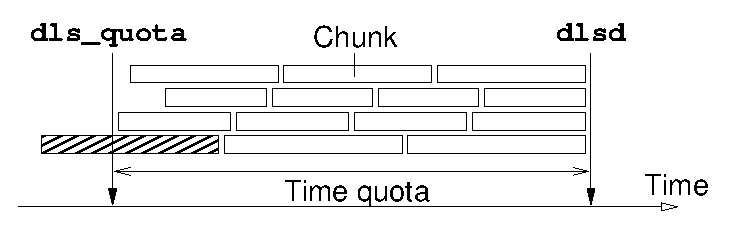
\includegraphics[width=250pt]{bilder/quota_en}
 \end{center}
 \caption{Compliance with the time quota}
 \label{fig:quota}
\end{figure}

Since the DLS quota daemon can always only remove complete chunks\index{chunk}
all at once, a successive deletion would not be possible, if the acquired data
of a channel consisted of one single chunk only. Therefore, it must be ensured
that always many small chunks exist, even if the dlsd acquisition process has
not been interrupted.

Hence, the dlsd acquisition process monitors the quota criteria for itself.
With the quota activated it makes sure that always sufficient individual
chunks are produced within the critical span (\autoref{fig:quota}). For this
purpose it splits every set quota criterion into equal portions and
independently begins a new chunk whenever one of these finer criteria is
exceeded.

As the completion of a chunk\index{chunk} may be very time-consuming, which is
incompatible with the real-time requirement of the dlsd acquisition process, a
dedicated process is generated for storing the remaining, acquired data. This
``clean-up process''\index{clean-up process} will now store all the data of
the current chunk, while the acquisition process simply discards them and
addresses the acquisition of the data of the newly started chunk. After
completion of the ``old'' chunk the clean-up process will quit automatically.

%------------------------------------------------------------------------------

\subsection{Messages from the data source}
\label{sec:dlsd_logger_msg}

The data source can -- in addition to the measured data -- send
messages\index{messages} at all times. These messages contain notes of the
user to be included in the data stream, warnings or error conditions. Messages
are of the following types:

\begin{description}

\item[info] - Information that is merely intended for the current acquisition
process.

\item[warn] - A warning from the data source.

\item[error] - An error occurred in the data source.

\item[crit\_error] - An error rendering further operation difficult or
impossible has occurred in the data source.

\item[broadcast] - A message for all processes that are currently connected
with the data source.

\end{description}

A message is always sent by the data source as a single XML tag, whose title
includes the type of the message. Moreover, the title contains an
attribute\textit{time} indicating the time stamp of the message in seconds and
- according to the message - an attribute \textit{text}, which will not be
evaluated any further by the dlsd.

A typical messages tag looks as follows:

\begin{lstlisting}
<broadcast time="1093072549.866241" text="test message"/>
\end{lstlisting}

The dlsd acquisition process stores the messages in the subdirectory
\textit{messages} of the job directory (see \autoref{sec:data_msg}). Just like
the measured data, messages are organised in chunks. The chunk concept,
however, has somewhat been modified here: Chunks that contain messages are not
continuous in terms of time and are created only to allow simpler deletion of
certain time spans from messages later on.

%------------------------------------------------------------------------------

\subsection{Signal processing}
\label{sec:dlsd_logger_signals}

The following signals\index{signal processing} are processed by the dlsd acquisition process:

\begin{description}

\item[SIGINT/SIGTERM] The acquisition process is to be terminated. Hereupon,
it will immediately terminate the connection to the data source and save the
data remaining in the memory to the hard disc. This may take a few seconds, as
possibly a lot of files needs to be written. If no error occurs in the
process, the process will quit with a return value of 0.

\item[SIGHUP] When receiving this signal, the acquisition process must newly
read in its specification data. Subsequently, it will check at once, whether -
according to the new specifications - it must continue to acquire data at all.
If not, it will initiate the termination as is done with \textit{SIGINT} or
\textit{SIGTERM}. Otherwise, it will send potentially changed specifications
to the data source and continue to acquire data after confirmation (see
\autoref{sec:dlsd_logger_comm}) under the new conditions.

\item[SIGCHLD] A ``clean-up process''\index{clean-up process} (see
\autoref{sec:dlsd_logger_quota}) has quit. This will only be registered via
the \textit{syslogd}\index{syslogd}.

\item[SIGSEGV and others] Treatment as in the parent process (see
\autoref{sec:dlsd_mother_signals}).

\end{description}

%------------------------------------------------------------------------------

\chapter{The DLS data directory}
\label{sec:data}

All persistent data of the DLS system are organised in \textit{DLS data
directories}\index{DLS data directory}. The basic structure is shown in
\autoref{fig:dls_data}.

\begin{figure}[htb] \begin{center} 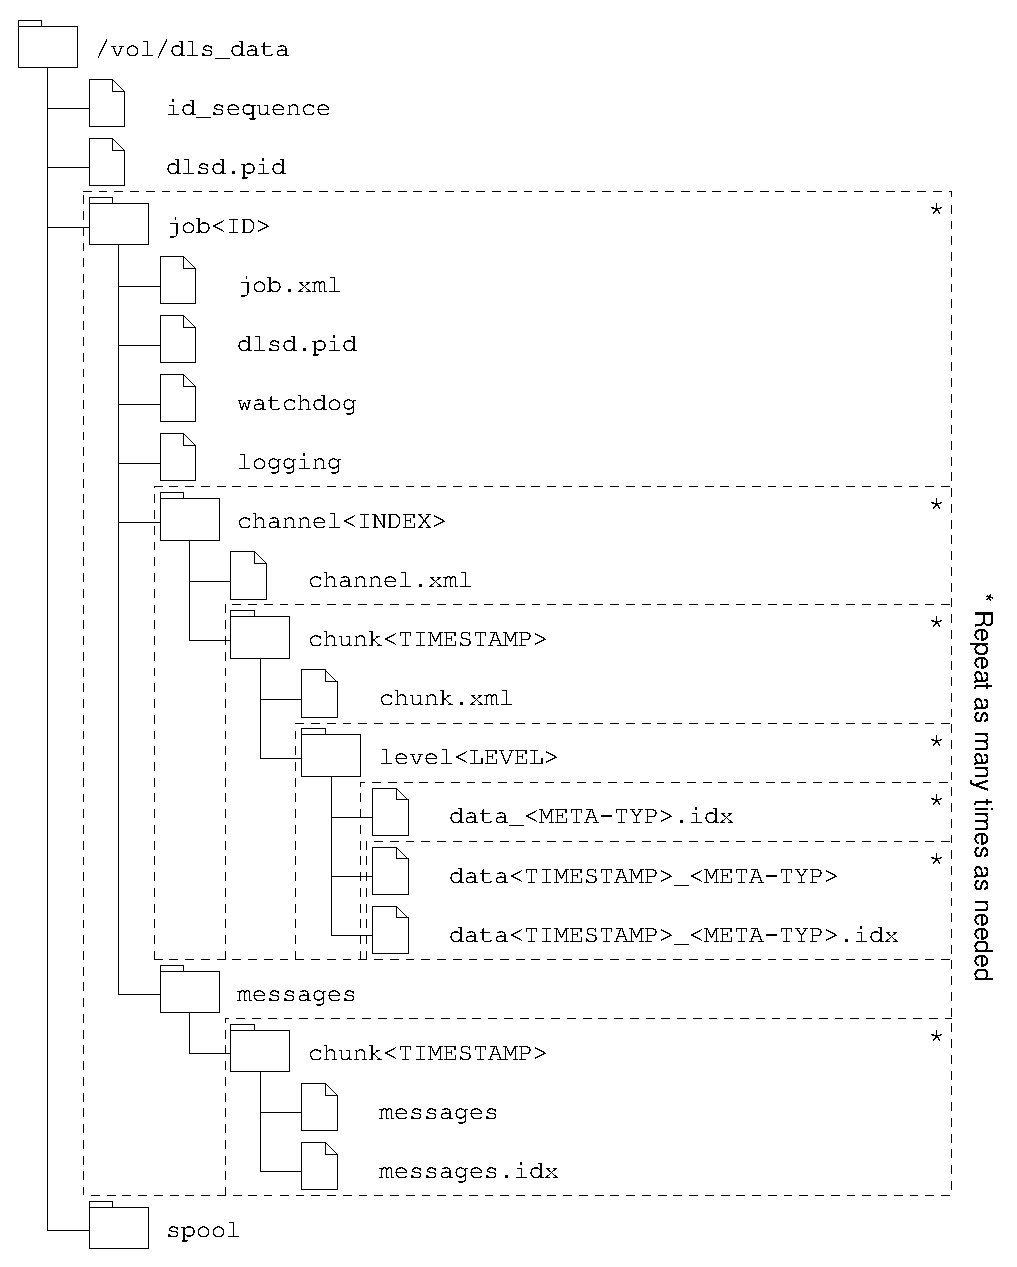
\includegraphics[width=300pt]{bilder/dls_data_en} \end{center} \caption{Structure of the DLS data directory} \label{fig:dls_data} \end{figure}

%------------------------------------------------------------------------------

\section{Root directory}
\label{sec:data_root}

The root directory is the topmost directory level within the DLS data
directory. Most of the files contained here belong to the dlsd parent process.
In addition, the root directory comprises all job directories (see
\autoref{sec:data_jobs}).

Files and subdirectories in the root directory:

\begin{description}

\item[id\_sequence] This file contains the next free job ID in the form of an
ASCII-coded digit sequence. This is required by the DLS Manager when a new job
is to be created. The DLS Manager reads the ID, uses it for the new job,
increases it by 1 and writes the new ID back to the file.

\item[dlsd.pid] This is the \textit{PID}file\index{PID files} of the dlsd
parent process (see \autoref{sec:apx_pid}). It is automatically created at
runtime and indicates that a dlsd parent process is running.

\item[jobXXX] Each job directory is available in the DLS root directory. The
name is always \textit{job}, followed by the job ID. See
\autoref{sec:data_jobs}.

\item[spool] This is the spooling directory of the dlsd parent process. A
description is given in \autoref{sec:dlsd_mother_spooling}.

\end{description}


%------------------------------------------------------------------------------

\section{Job directories}
\label{sec:data_jobs}

During on-going operation, every job directory (\textit{job\textless ID\textgreater}) is processed by a dedicated dlsd acquisition process. The latter reads its specifications from there and also writes the acquired data there.

Files and subdirectories in a job directory:

\begin{description}

\item[job.xml] The central specifications file for a job. It contains job and
channel specifications. If it is edited while the pertaining acquisition
process is running, a spooling command (see
\autoref{sec:dlsd_mother_spooling}) must be generated in order to have the
process adopt the new specifications. The DLS Manager will automatically do
this.

The specifications file in XML format contains the following information (order being compulsory!):

\begin{lstlisting}
<dlsjob>
 <description text="`\textit{description}`"/>
 <state name="`\textit{(}`running`\textit{|}`paused`\textit{)}`"/>
 <source address="`\textit{IP address or host name}`"/>
 <quota size="`\textit{data quota}`" time="`\textit{time quota}`"/>
 <trigger parameter="`\textit{trigger parameter}`"/>

 <channels>
  <channel name="`\textit{channel name}`" `$\hookleftarrow$`
   frequency="`\textit{sampling frequency}`" `$\hookleftarrow$`
   block_size="`\textit{block size}`" `$\hookleftarrow$`
   meta_mask="`\textit{meta mask}`" `$\hookleftarrow$`
   meta_reduction="`\textit{meta reduction ratio}`" `$\hookleftarrow$`
   format="`\textit{compression format}`" `$\hookleftarrow$`
   mdct_block_size="`\textit{MDCT block size}`" `$\hookleftarrow$`
   mdct_accuracy="`\textit{MDCT accuracy}`" `$\hookleftarrow$`
   type="`\textit{data type}`"/>
 </channels>
</dlsjob>
\end{lstlisting}

The attributes \textit{mdct\_block\_size} and \textit{mdct\_accuracy} will
only be required when the compression format is based on the MDCT (see
\autoref{sec:comp_mdct}).

The specifications can be edited with the DLS Manager. The individual
parameters are described in \autoref{sec:manager_auftrag_create} and
\autoref{sec:manager_kanaele_edit}.

\item[watchdog and logging] These are two empty files used for the DLS
Manager’s monitoring of the dlsd acquisition processes. If an acquisition
process is running for the job directory, it will change the time stamp of the
\textit{watchdog} file every second. If the process is simultaneously
acquiring data, it will likewise proceed with the \textit{logging} file. The
DLS Manager checks the time stamps of these files in regular intervals, will
thus receive information about the condition of the acquisition process and
will thus be able to display it to the user.

\item[dlsd.pid] This is the \textit{PID}file\index{PID files} of the dlsd
acquisition process (see \autoref{sec:apx_pid}). It is automatically created
at runtime and indicates that a dlsd acquisition process is running.

\item[channelXXX] The acquired data continue to be organised in channels that
have their own channel directory each (see \autoref{sec:data_channels}).  The
index in the name of the channel directory corresponds to the channel index
that the \textit{\textless rk\textgreater}  command has returned when it reads
out all the channels of the data source during the starting process of the
dlsd parent process (see \autoref{sec:dlsd_logger_comm}).

\item[messages] Every acquisition process stores the messages, which it has
received from the data source during the data acquisition, to this directory.
If it does not yet exist, the process will create it when required. Just like
the measured data, messages are organised in chunks. See
\autoref{sec:data_msg}.

\end{description}


%------------------------------------------------------------------------------

\section{Channel directories}
\label{sec:data_channels}

All the data that have been acquired for a certain channel are filed in the channel directories (\textit{channel\textless INDEX\textgreater}). A channel directory is permanently assigned to a specific channel of the data source. For the description of the channel’s properties, there is the file \textit{channels.xml} with the following contents:

\begin{lstlisting}
<dlschannel>
 <channel name="`\textit{channel name}`" index="`\textit{Index}`" `$\hookleftarrow$`
  unit="`\textit{unit}`" type="`\textit{Datentyp}`"/>
</dlschannel>
\end{lstlisting}

This file serves not only for the description of the data in the chunk directories but will also be checked by the dlsd acquisition process each time a new data acquisition is to be made in a channel directory. This shall take place only if the channel data (name, index, unit and type) have not changed.

%------------------------------------------------------------------------------

\section{Chunk directories}
\label{sec:data_chunks}

The acquired data of a channel are organised in \textit{chunks}
(\textit{chunk\textless TIME\textgreater}). A chunk\index{chunk} is a
completely acquired series of data which were acquired with the same
channel specification as from a certain point in time. The time stamp
in the directory is the time stamp of the first data value in the
chunk. For the description of the chunk's properties, there is the
file \textit{chunk.xml} with the following contents:

\begin{lstlisting}
<dlschunk>
 <chunk sample_frequency="`\textit{Abtastrate}`" `$\hookleftarrow$`
  block_size="`\textit{Datenblockgröße}`" `$\hookleftarrow$`
  meta_mask="`\textit{Meta-Maske}`" `$\hookleftarrow$`
  meta_reduction="`\textit{Meta-Untersetzung}`" `$\hookleftarrow$`
  format="`\textit{Kompressionsformat}`" `$\hookleftarrow$`
  mdct_block_size="`\textit{MDCT-Blockgröße}`" `$\hookleftarrow$`
  mdct_accuracy="`\textit{MDCT-Genauigkeit}`" `$\hookleftarrow$`
  architecture="`\textit{Architektur (Endianess)}`"/>
</dlschunk>
\end{lstlisting}

The \textit{mdct\_*}-Attribute attributes will exist only if the compression
format is based on the MDCT (see \autoref{sec:comp_mdct}).

In each chunk directory the data are accommodated in directories that correspond to their meta level (generic data in the \textit{level0} directory, data of the first meta level in the \textit{level1} directory etc.).

%------------------------------------------------------------------------------

\section{Data directories}
\label{sec:data_data}

The data directories (\textit{level\textless meta level\textgreater}), which simultaneously represent the sorting of the data according to the respective meta level, are arranged at the bottom of the directory hierarchy. The data files and the associated index files are provided here.

\paragraph{Data files} Data files contain the acquired measured data. These are created separately for each meta type. Therefore, the file has the following naming convention:

\begin{quote} \textit{data\textless TIMESTAMP\textgreater\_\textless METATYPE\textgreater} \end{quote}

The time stamp in the file name is the time stamp of the first data value in the first block in this file.

In the \textit{level0} directory the meta type is always \textit{gen} (``generic'').

Data files have a simple XML structure. Each data block appears as a \textit{\textless d\textgreater}-Tag. This contains the time stamp of the first value in the block as attribute \textit{t} (``time''), the number of compressed data values as attribute \textit{s} (``size'') and the coded data as attribute \textit{d}(``data'').

Data files have a defined maximum size. As soon as the dlsd acquisition process exceeded that size by adding the next block, it would first create a new data file.

The facts which parameters have ultimately been used for the data acquisition and in which way the compression has taken place can only be determined together with the higher-ranking description files \textit{chunk.xml} and \textit{channel.xml}.

\paragraph{Index files} Index files are binary files with a fixed entry length, which are always assigned to a data file. They provide information that can very quickly be read out, about the data blocks in the corresponding data file. The naming convention is similar to that of the data file, but with an additional extension:

\begin{quote} \textit{data\textless TIMESTAMP\textgreater\_\textless METATYPE\textgreater.idx} \end{quote}

The entries in the index file will always correspond to a block in the data
file. The structure of an entry is shown in \autoref{fig:dls_data_index}.

\begin{figure}[htb] \begin{center} 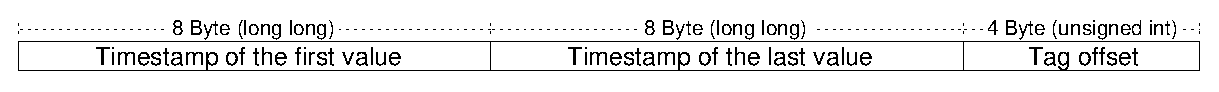
\includegraphics[height=15pt]{bilder/dls_data_index_en} \end{center} \caption{Entry of an index file} \label{fig:dls_data_index} \end{figure}

Each entry is 20 bytes long. The first 8 bytes correspond to the time stamp of
the first data value in the respective block in microseconds, which has been
converted into a \textit{long long int}. The next 8 bytes correspond in the
same way to the time stamp of the last data value in the block. The last 4
bytes are the \textit{unsigned int}-coded offset address of the block tag in
the data file, i.\,e. the position of the initial \textit{\textless}
character.

\paragraph{Global index files} ``Global'' index files facilitate the
determination of the time spans of the data of individual data files of a
certain meta type. Their naming convention is:

\begin{quote} \textit{data\_\textless METATYPE\textgreater.idx} \end{quote}

An entry in a global index file will always correspond to a data file of the
same meta type. The structure of an entry is shown in
\autoref{fig:dls_data_index_glob}.

\begin{figure}[htb] \begin{center} 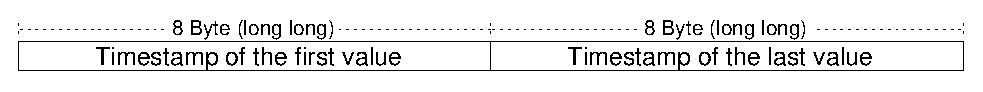
\includegraphics[height=15pt]{bilder/dls_data_index_glob_en} \end{center} \caption{Entry of a global index file} \label{fig:dls_data_index_glob} \end{figure}

An entry in a global index file is always 16 bytes long. The first 8 bytes correspond to the time stamp of the first data value in the data file in microseconds as a \textit{long long int}, the last 8 bytes correspond to the last data value.

If data are just being entered in a data file, the time stamp of the corresponding (latest) entry in the global index file will be 0. In this case the searched time stamp must be ascertained by reading out the latest entry in the corresponding data index file. As soon as the data acquisition in the data file is terminated, the second time stamp will be given the ``correct'' value.

%------------------------------------------------------------------------------

\section{Messages directory}
\label{sec:data_msg}

Messages from the data source are stored in the messages directory (\textit{messages}) in separated chunks. All the chunk directories are designated with

\begin{quote} \textit{chunk\textless TIMESTAMP\textgreater}, \end{quote}

with the time stamp corresponding to that of the first message recorded in this directory. Within the directories there are always only two files: the message file and the associated message index file.

\paragraph{Message files} A file with messages from the data source is always
denominated as \textit{messages}. The messages of the data source are stored
unchanged in this file, so that this contains only single SML tags that
correspond to the respective messages (see \autoref{sec:dlsd_logger_msg}).

\paragraph{Message index files} The index file \textit{messages.idx} belongs to the message file proper and serves to enable the quick loading of messages of a certain time range without having to read in the whole message file.

An entry in a message index file will always correspond to a message in the
message file. The structure of an entry is shown in
\autoref{fig:dls_data_index_msg}.

\begin{figure}[htb] \begin{center} 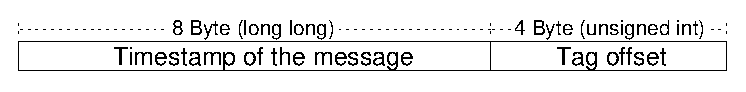
\includegraphics[height=15pt]{bilder/dls_data_index_msg_en} \end{center} \caption{Entry of a message index file} \label{fig:dls_data_index_msg} \end{figure}

%------------------------------------------------------------------------------

\chapter{The DLS Manager}
\label{sec:manager}

The \textit{DLS Manager}\index{DLS Manager} is the graphical user interface for the configuration of the measurement jobs\index{measurement job} in a DLS data directory. Furthermore, it serves for the control and monitoring of the running acquisition processes.

The DLS Manager is called with the command \texttt{dls\_ctl}.

Same as for the dlsd, in the command line, with the parameter \texttt{-d},
this tool can be notified of the DLS data directory, in which it is to work
(see \autoref{sec:apx_cmd_dlsctl}).

When the program is started the DLS Manager automatically performs some checks:

\begin{itemize}
\item If the DLS data directory involved is still empty, the user will be asked whether a valid DLS data directory structure is to be created in the directory.
\item If for the DLS data directory involved an instance of the dlsd is not yet running, the user will be asked whether an instance is to be started. \end{itemize}

%------------------------------------------------------------------------------

\section{Main dialog}

\autoref{fig:dls_ctl_main} shows the main window of the DLS Manager, which
will be displayed once the program is started.

\begin{figure}[tbh] \begin{center} 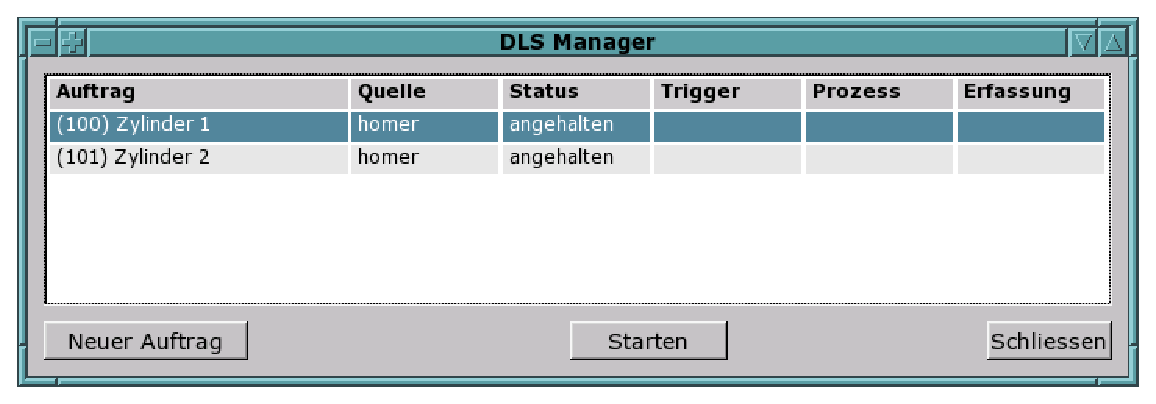
\includegraphics[width=300pt]{bilder/ctl_main} \end{center} \caption{Main dialog of the DLS Manager} \label{fig:dls_ctl_main} \end{figure}

%------------------------------------------------------------------------------

\subsection{Display features}

In the main dialog the individual measurement jobs\index{measurement job} are
displayed as lines in a table. The following information is made available in
the columns:

\begin{description}
\item[Job ID and designation] The designation of the job is arbitrary and can be changed at any time. The ID is a fixed number automatically chosen when creating the job. All data of a job are stored in the DLS data directory in subdirectory \textit{job\textless ID\textgreater}.
\item[Source] The name or the IP address of the server that is to be
  used as the data source. On this an I\&C server must be accessible
  via the TCP port 2345. The source can be chosen only when creating
  the job and cannot be changed later on.
\item[Status] The job status selected by the user: ``started'', when the data acquisition is to run, otherwise ``stopped''.
\item[Trigger]. The parameter of the data source that is to serve the acquisition process as trigger parameter. Where a trigger parameter has been selected, data will be acquired only, if this has the value 1.
\item[Process] Indicates whether an acquisition process is currently running for this job. Is not displayed when the job has been stopped.
\item[Acquisition] If a trigger has been configured, here you can see, whether this is currently switched on. Without trigger, the data acquisition must always run when the acquisition process is running. \end{description}

%------------------------------------------------------------------------------

\subsection{Interaction features}

\begin{itemize}

\item The lines containing the individual jobs can be marked with the mouse
cursor.

\item When a job has been marked, a button to start or stop the data
acquisition will be displayed.

\item A double click on a job line opens the dialog for editing the respective
job (see \autoref{sec:manager_auftrag_edit}).

\item The button ``Close'' terminates the program.

\end{itemize}

%------------------------------------------------------------------------------

\section{The ``Create job'' and ``Change job'' dialogs}
\label{sec:manager_auftrag_create}

\autoref{fig:dls_ctl_change} shows the dialog for creating or changing a
measurement job. It is displayed after clicking the buttons ``New job'' in the
main dialog or ``Change'' in the ``Edit job''.  dialog. They differ in that
the data source can only be changed when creating a job.

\begin{figure}[tbh] \begin{center} 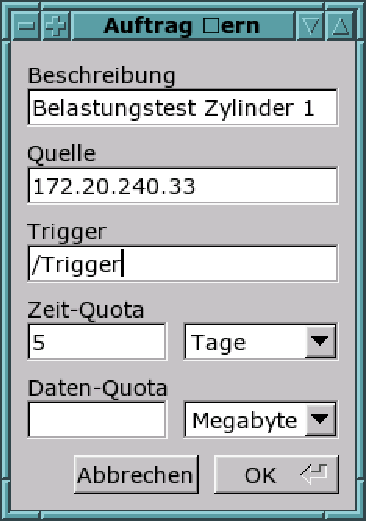
\includegraphics[width=100pt]{bilder/ctl_change} \end{center} \caption{Dialog for creating or changing a measurement job} \label{fig:dls_ctl_change} \end{figure}

%------------------------------------------------------------------------------

\subsection{Display features}

The dialog mask enables the user to indicate several particulars regarding the measurement job:

\begin{description}

\item[Description] This is an arbitrary name for the measurement job, which is
merely used for recognition purposes.

\item[Source] The address of the data source. This may be a host name or an IP
address. If a host name is used, it must be ensured that at runtime it can be
resolved by the dlsd into an IP address. The specified host must provide a
data source for the data acquisition and for the addition of channels via the
corresponding dialog (see \autoref{sec:manager_kanaele_hinzu}).

\item[Trigger] The name of the parameter that is to serve as the trigger
parameter. If a trigger parameter\-meter  has been selected here, data will
later be acquired only, if this has the value 1. If this input field is left
empty, no trigger will be used.

\item[Time quota] The time quota (duration of the period of time to be
maximally stored for acquired data, see \autoref{sec:dlsd_logger_quota}) can
be set here as a combination of an (integer) value and the associated time
unit. No entry in the input field for the value means that no time quota is to
be used.

\item[Data quota] Here, the data quota (amount of storage space to be
maximally used and to be reserved in the file system for the acquired data)
can also be indicated as a combination of an integer and the associated unit
of size. Again, no entry means that no data quota is to be used.

\end{description}

%------------------------------------------------------------------------------

\subsection{Interaction features}

\begin{itemize}
\item Clicking the ``OK'' button (or pressing the \textit{Enter} key) will verify the specified data. If these contain errors, a window with the exact error messages will be displayed. Otherwise, the data will be accepted and the dialog closed. If a dlsd acquisition process is running, it will be requested to take over the new specifications.
\item If the ``Cancel'' button is clicked, the specified data will be discarded and the dialog closed. \end{itemize}

%------------------------------------------------------------------------------

\section{The ``Edit job'' dialog}
\label{sec:manager_auftrag_edit}

\autoref{fig:dls_ctl_edit} shows the dialog for editing a job, which will be
displayed in the main dialog window after having double-clicked on a job.

\begin{figure}[tbh] \begin{center} 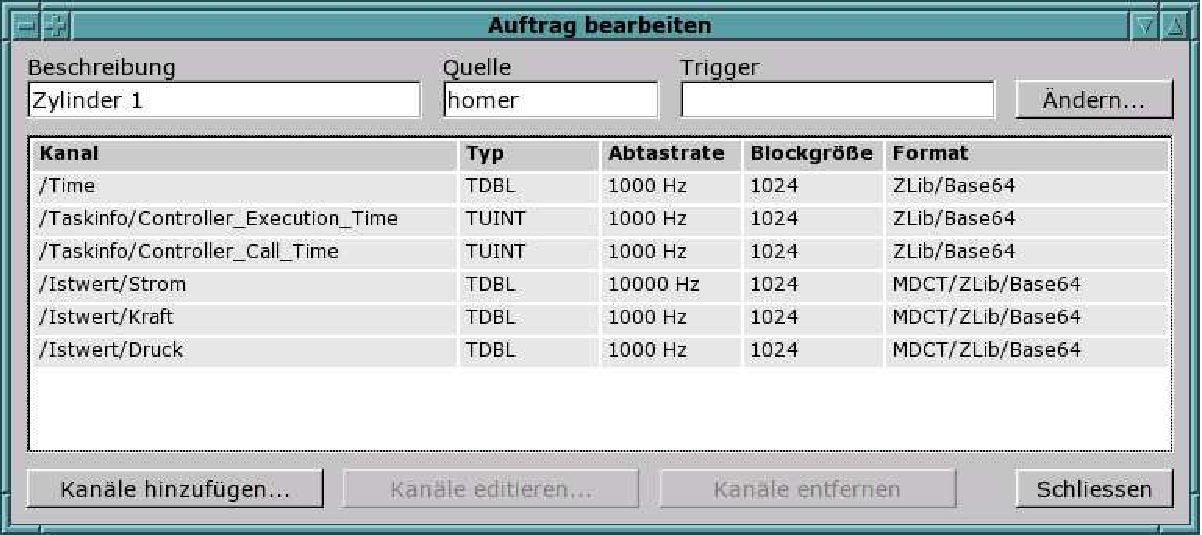
\includegraphics[width=300pt]{bilder/ctl_edit} \end{center} \caption{Dialog for editing a job} \label{fig:dls_ctl_edit} \end{figure}

%------------------------------------------------------------------------------

\subsection{Display features}

Selected master data of the job are displayed in the top section. Below there is the list of the channels to be included with the key parameters. These are in particular:

\begin{description}

\item[Channel] The name of the channel to be included

\item[Type] The channel type. A channel can either be of an integer or a
floating-point type (see \autoref{sec:apx_types}).

\item[Scanning frequency] The frequency, with which the individual measured
values are to be stored.

\item[Block size] The number of measured values that are to be jointly
compressed and saved in one unit.

\item[Format] The compression method (see \autoref{sec:comp}).

\end{description}

%------------------------------------------------------------------------------

\subsection{Interaction features}

\begin{itemize}

\item The dialog for editing the job’s master data can be called up by
clicking the ``Change'' button.

\item The channel lines of the table can be marked with the mouse cursor. It
will then be possible to use the ``Edit channels'' and ``Delete channels''
buttons.

\item By pressing the \textit{Shift} or \textit{Ctrl} key you may also select
several channels at a time, which will be simultaneously editable and
deletable as well.

\item The specifications for one or more highlighted channels can be edited by
clicking the ``Edit channels.'' buttons in the following dialog. Special
conditions apply, however, for the editing of several channels (see
\autoref{sec:manager_kanaele_edit_parallel}).

\item A double click on a channel line will also open the dialog for editing
the specifications of the respective channel.

\item If the ``Delete channels'' button is clicked, all highlighted
channels will be removed from the specifications. Any data acquired,
however, will remain available.

\item When the ``Add channels'' button is clicked, the dialog for the adding
of channel specifications will open (see \autoref{sec:manager_kanaele_hinzu}).

\item The ``Close'' button terminates the dialog and returns to the main
dialog.

\end{itemize}

%------------------------------------------------------------------------------

\section{The ``Add channels'' dialog} \label{sec:manager_kanaele_hinzu}

Upon clicking the ``Add channels'' button in the dialog for editing a job, a
dialog window will open as shown in \autoref{fig:dls_ctl_add}. At the same
time it is tried to establish a TCP connection to the data source to retrieve
its channels.

\begin{figure}[tbh] \begin{center} 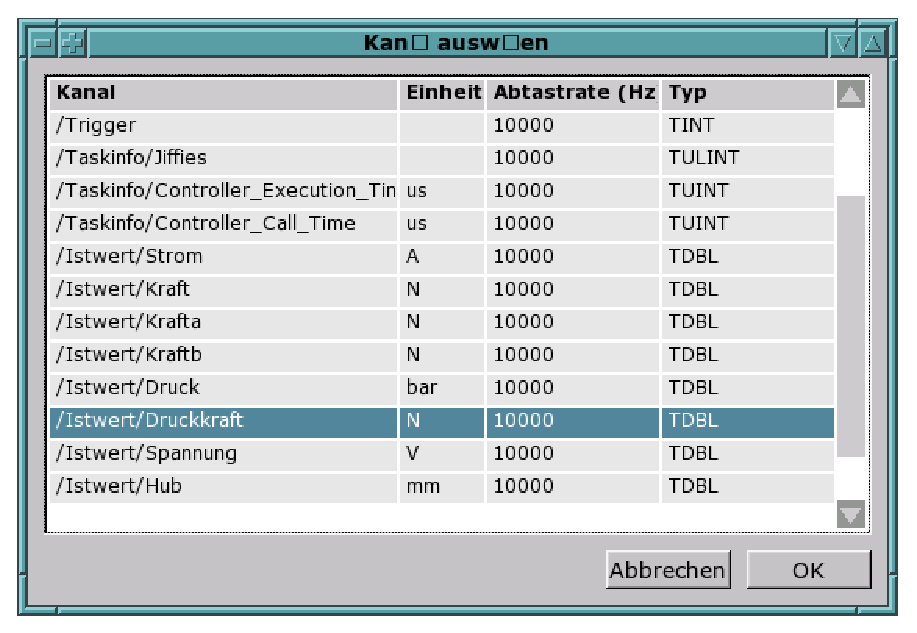
\includegraphics[width=300pt]{bilder/ctl_add} \end{center} \caption{Dialog for adding channel specifications} \label{fig:dls_ctl_add} \end{figure}

%------------------------------------------------------------------------------

\subsection{Display features}

\begin{itemize}
\item While it is tried to establish the connection with the data source, a ``Receiving channels\ldots''.  message is displayed. If even after a defined waiting time the connection still fails to be established, a window with the corresponding error message will appear and the dialog will close.
\item If the channel list has successfully been accessed, the individual channels will be displayed in a table. The channel name, the unit, the maximum sampling frequency and the channel data type will be shown. \end{itemize}

%------------------------------------------------------------------------------

\subsection{Interaction features}

\begin{itemize}

\item The user can use the cursor to select individual channels. By pressing
the \textit{Ctrl} or \textit{Shift} key it is possible to select several
channels at the same time.

\item When the ``OK'' button is clicked, all selected channels will be added
to the list of the job’s channel specifications. If a certain channel is
already available, this will be shown in a window with the corresponding
warning message. The other channels will be added nevertheless. If changes
have been made, a possibly running dlsd acquisition process will be requested
to adopt the new channel specifications.

\item Clicking the ``Cancel'' button will close the dialog without adding new
channel specifications to the job.

\end{itemize}

%------------------------------------------------------------------------------

\section{The ``Edit channels'' dialog} \label{sec:manager_kanaele_edit}

The dialog for the editing of channel specifications shown in
\autoref{fig:dls_ctl_channel} will appear when double clicking on a channel
specification in the dialog for the editing of a job, or after clicking the
``Edit channels'' button after one or more channels have been selected.

\begin{figure}[tbh] \begin{center} 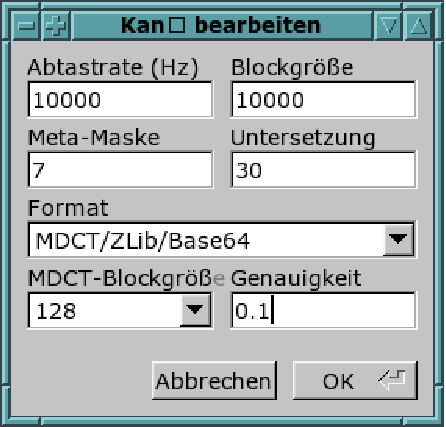
\includegraphics[width=100pt]{bilder/ctl_channel} \end{center} \caption{Dialog for editing channel specifications} \label{fig:dls_ctl_channel} \end{figure}

%------------------------------------------------------------------------------

\subsection{Display features}

The following input fields are available to the user for a parameterisation of the channel specification(s):

\begin{description}

\item[Abtastrate] The number of values to be stored per second. This frequency
must be an integer divisor of the maximum sampling frequency of the channel
concerned.

\item[Blockgröße] The number of values compressed and stored in a block. The
larger the block, possibly the better the compression result, but the longer
the duration of the compression process. For an MDCT-based compression the
block size must be an integer multiple of the MDCT block size.

\item[Meta mask] \textit{This value is currently not editable}\\ The meta mask
is a bit mask indicating the types of meta data to be stored. See
\autoref{sec:dlsd_data_meta} in this respect.

\item[Reduction ratio] The meta reduction ratio is the number of data values
of a meta level, from which a new meta value of the next higher level is
generated. In this respect, too, see \autoref{sec:dlsd_data_meta}. This value
usually does not require any adjustment.

\item[Format] The compression format, with which the acquired data are
compressed prior to storage. Depending on the compression method used, further
parameters need to be specified.

\item[MDCT block size] This parameter must be specified for MDCT-based
compression methods and behaves similar to the block size. See
\autoref{sec:comp_mdct}.

\item[Accuracy]  Some non lossless compression methods allow specifying the
maximum, absolute error. The error must always be indicated in the unit of the
corresponding channel.

\end{description}

%------------------------------------------------------------------------------

\subsection{Interaction features}

\begin{itemize} \item Clicking the ``OK'' button will first verify the
specified parameters for plausibility. If this fails, a window with the
relevant error messages will be displayed. Otherwise, all specified parameters
will be applied to the previously selected channel specifications, the
possibly running dlsd acquisition process will be requested to adopt the new
parameters and the dialog will be closed.  \item If the ``Cancel'' button is
clicked, the specified data will be discarded and the dialog closed.
\end{itemize}

%------------------------------------------------------------------------------

\subsection{Simultaneous editing of several channel specifications} \label{sec:manager_kanaele_edit_parallel}

The dialog for editing the channel specifications
(\autoref{fig:dls_ctl_channel}) can also be used for editing several channels
simultaneously. In this case the following applies:

\begin{itemize}
\item When opening the dialog, all parameters which at that time are identical regarding all channel specifications to be edited will be displayed in the dialog mask. In respect of the parameters that are \textbf{not} identical regarding all channel specifications, the corresponding input fields are left empty.
\item Accordingly, after having changed or added a value in the dialog mask, clicking the ``OK'' button will affect \textbf{all} previously selected channel specifications.
\item If a value field in the mask is empty when clicking ``OK'', that value will be changed for \textbf{none} of the channel specifications. In this case, all previously selected channels will retain the respective previous value. Thus, it is possible to change for example only the sampling frequency for a number of channel specifications.
\item The parameters of the compression (\textit{format}, \textit{MDCT block size} and \textit{accuracy}) are one unit in this regard. This means that initially the compression parameters will be displayed only, if they are exactly the same for \textbf{all} channel specifications. Accordingly, the specified compression parameters can also only be edited collectively. \end{itemize}

%------------------------------------------------------------------------------

\chapter{The DLS View} \label{sec:view} \index{DLS View viewer program}

The \textit{DLS View} program serves for the simple view of the acquired data
of a job. It is therefore made up of only two dialogs (see
\autoref{fig:dls_view_main} and \autoref{fig:dls_view_export}).

%------------------------------------------------------------------------------

\section{Main dialog} \label{sec:view_main}

\begin{figure}[tbh] \begin{center} 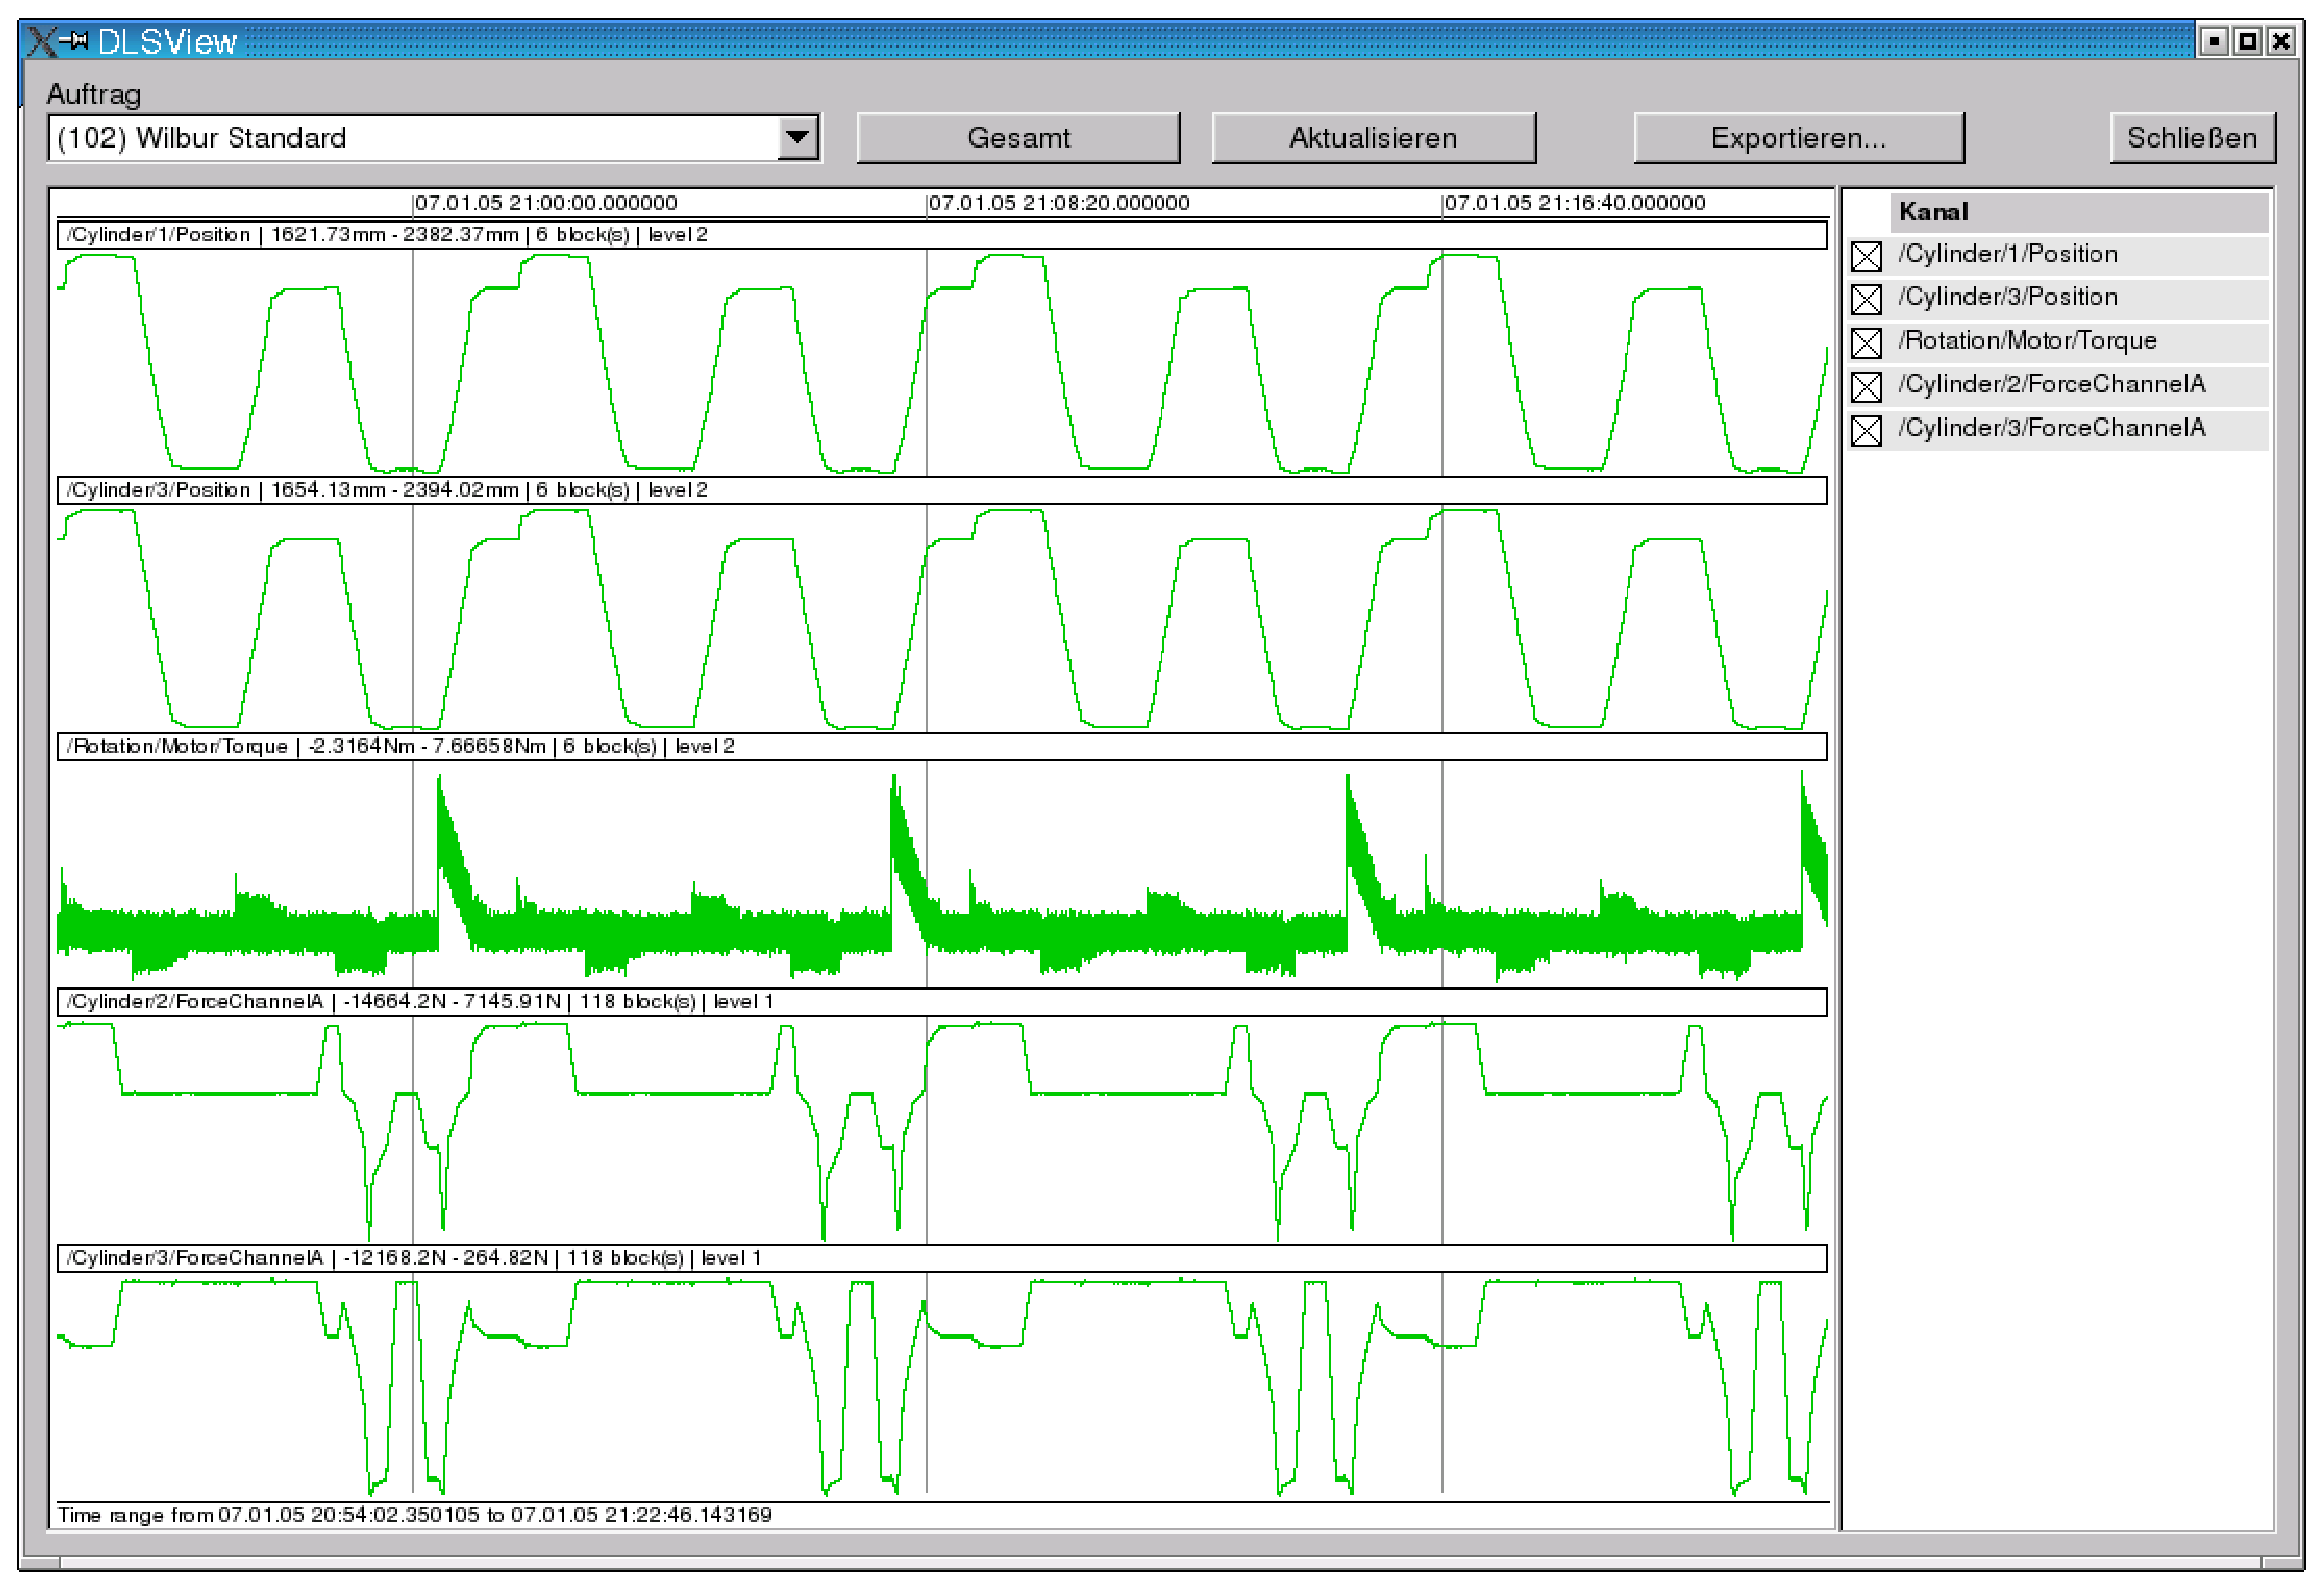
\includegraphics[width=\textwidth]{bilder/view_normal} \end{center} \caption{Main dialog of DLS View} \label{fig:dls_view_main} \end{figure}

%------------------------------------------------------------------------------

\subsection{Display features}

\begin{itemize}

\item At the top left corner of the screen there is a selection field where
the user can select the measurement job whose data are to be displayed.

\item On the right-hand side a list of the channels covered by the selected
job is displayed.

\item The biggest part of the dialog window is taken up by the data display.
Its design allows to display the data of several channels arranged one above
the other on a common time scale shown on top of the chart. The tick marks
appear as vertical, grey lines in a coordinate system.

\item In a small text line at the very bottom of the chart you see the
respective time range presented.

\item A small header above each channel contains the channel name, the
presented value range, the number of loaded data blocks and the loaded meta
level (see \autoref{sec:dlsd_data_meta}). Under the header the data are
represented in curves. A blue curve indicates that the data involved are
generic data (meta level 0); if a higher meta level is used for the
representation, the respective curve section is green.

\item If no data were acquired in a certain time span, this zone of the
channel line concerned is displayed with a yellow background (see
\autoref{fig:dls_view_scan}).

\item As all channel lines must share the overall height of the display, with
an increasing number of channels to be displayed the height of the individual
channel lines decreases. If the height of an individual channel line falls
below a defined value, a scroll bar will appear on the right.

\end{itemize}

%------------------------------------------------------------------------------

\subsection{Interaction features}

\begin{itemize}

\item From the selection list ``Job'' the user can choose the job whose
acquired data he wants to have displayed. The list of acquired channels will
then be updated.

\item The user can hide or display individual channels in the data display by
ticking the box in front of the respective channel names in the channel list.

\item Clicking on the ``All'' button will determine and display the entire
time range, in which data have been acquired for the selected channels.

If channels are added or deleted immediately thereafter, the new entire time
range will be determined time and again. Only when the user explicitly selects
another time range to be displayed, such range will be constantly applied even
if channels are added or deleted.

\item Clicking on the ``Update'' button will have all channel data of the
selected time range re-recorded and displayed.

\item When clicking on the ``Export\ldots'' button, the export dialog (see
\autoref{sec:view_export}) will open.

\item Through pressing and holding the left mouse button within the data area
of the display the user can select a new time range which will remain marked
by two vertical red lines as long as the mouse button is held down. Their
exact points in time are indicated at the top edge of the chart. When
releasing the left mouse button the new time range will be accepted and the
corresponding data loaded.

By the way, when releasing the mouse button the position may well lay outside
the display range, which will then result in a slight extension of the
displayed time span.

\item Similarly, by pressing and holding the right mouse button on the display
range the time span presented can be moved. When the mouse button is released,
the new time range is accepted.

\item A double click in the data area results in the time range presented
being extended by the factor 2. Before that, it is centred around the point in
time just clicked. If the \textit{Shift} button is being pressed while double
clicking, the factor 10 will be used for the extension.

\item If the data area has the keyboard focus, pressing the
\textit{Ctrl}button will draw a vertical ``scan line'' at the point in time to
which the mouse cursor points (see \autoref{fig:dls_view_scan}). If this line
crosses a displayed curve, the data value at the point of intersection will be
displayed.

As the scan line is not infinitely narrow, possibly many data values will fall
in the area covered by it. In this case the entire value area of the values
that are present ``under'' the scan line will be marked by two horizontal
lines corresponding to the minimum and maximum (see 3rd channel in
\autoref{fig:dls_view_scan}).

\end{itemize}

\begin{figure}[tbh] \begin{center} 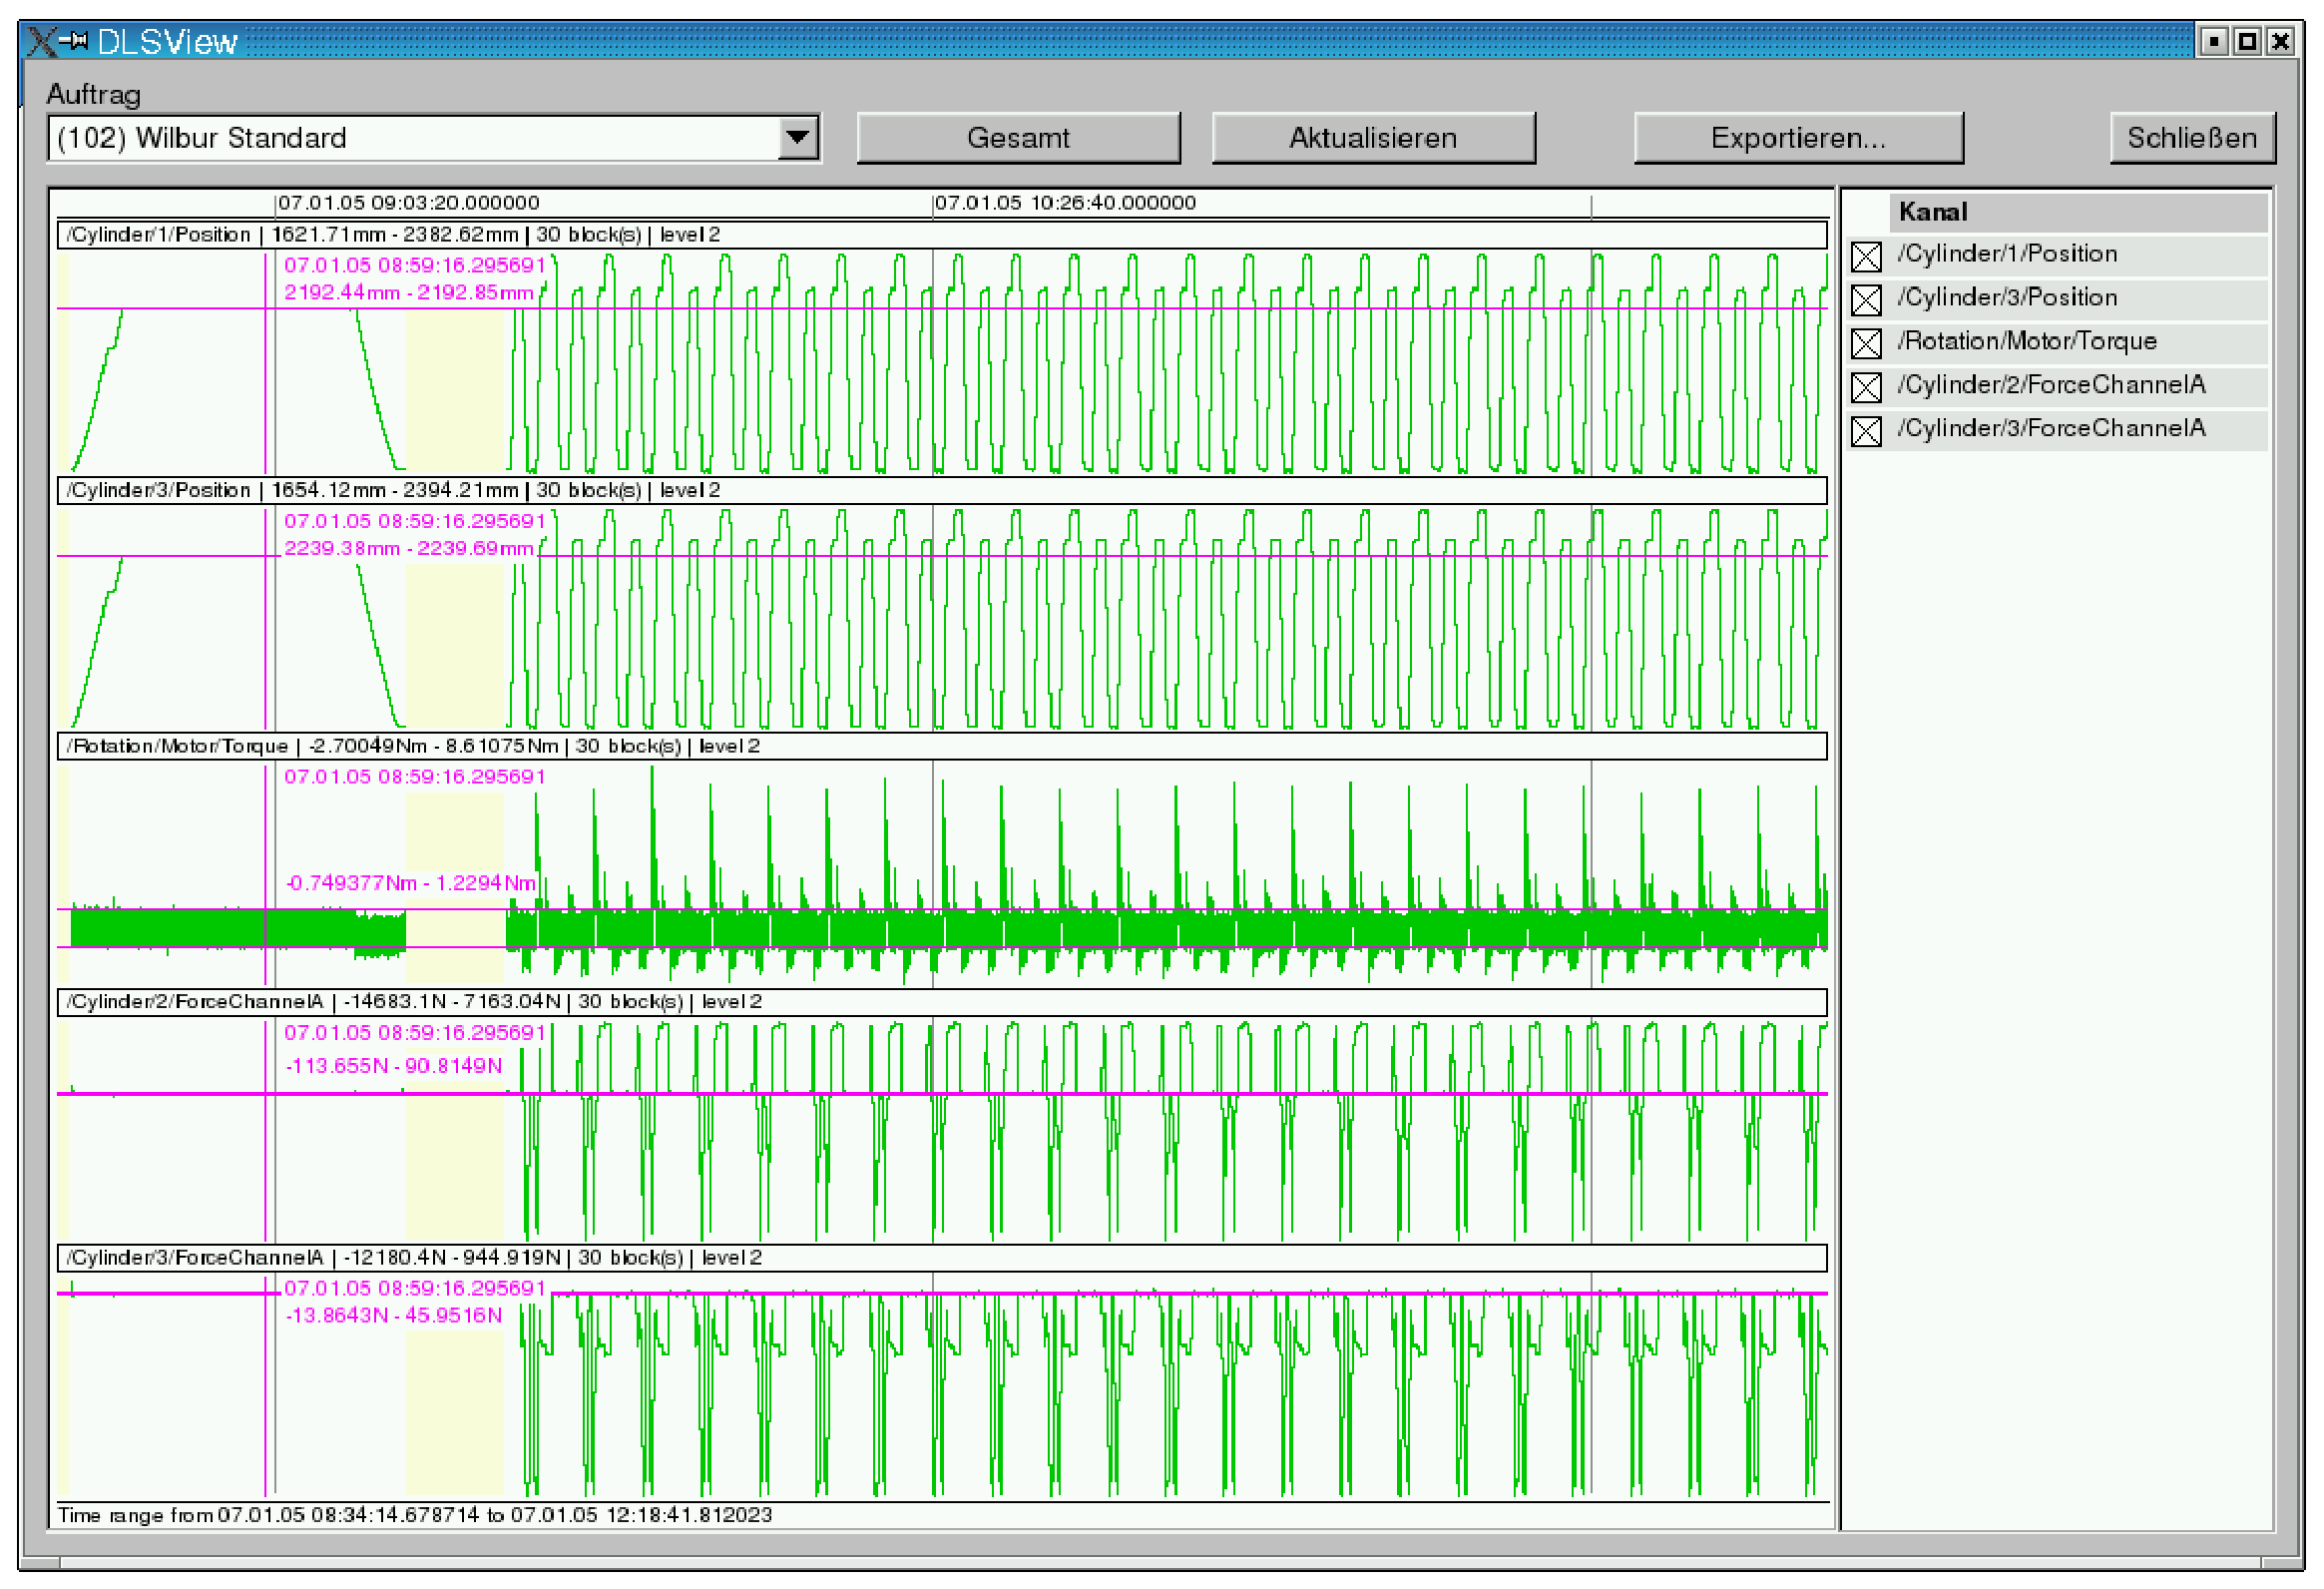
\includegraphics[width=\textwidth]{bilder/view_scan} \end{center} \caption{Scan lines with the \textit{Ctrl}button held down} \label{fig:dls_view_scan} \end{figure}

%------------------------------------------------------------------------------

\section{The ``Export\ldots'' dialog} \label{sec:view_export}

\begin{figure}[tbh] \begin{center} 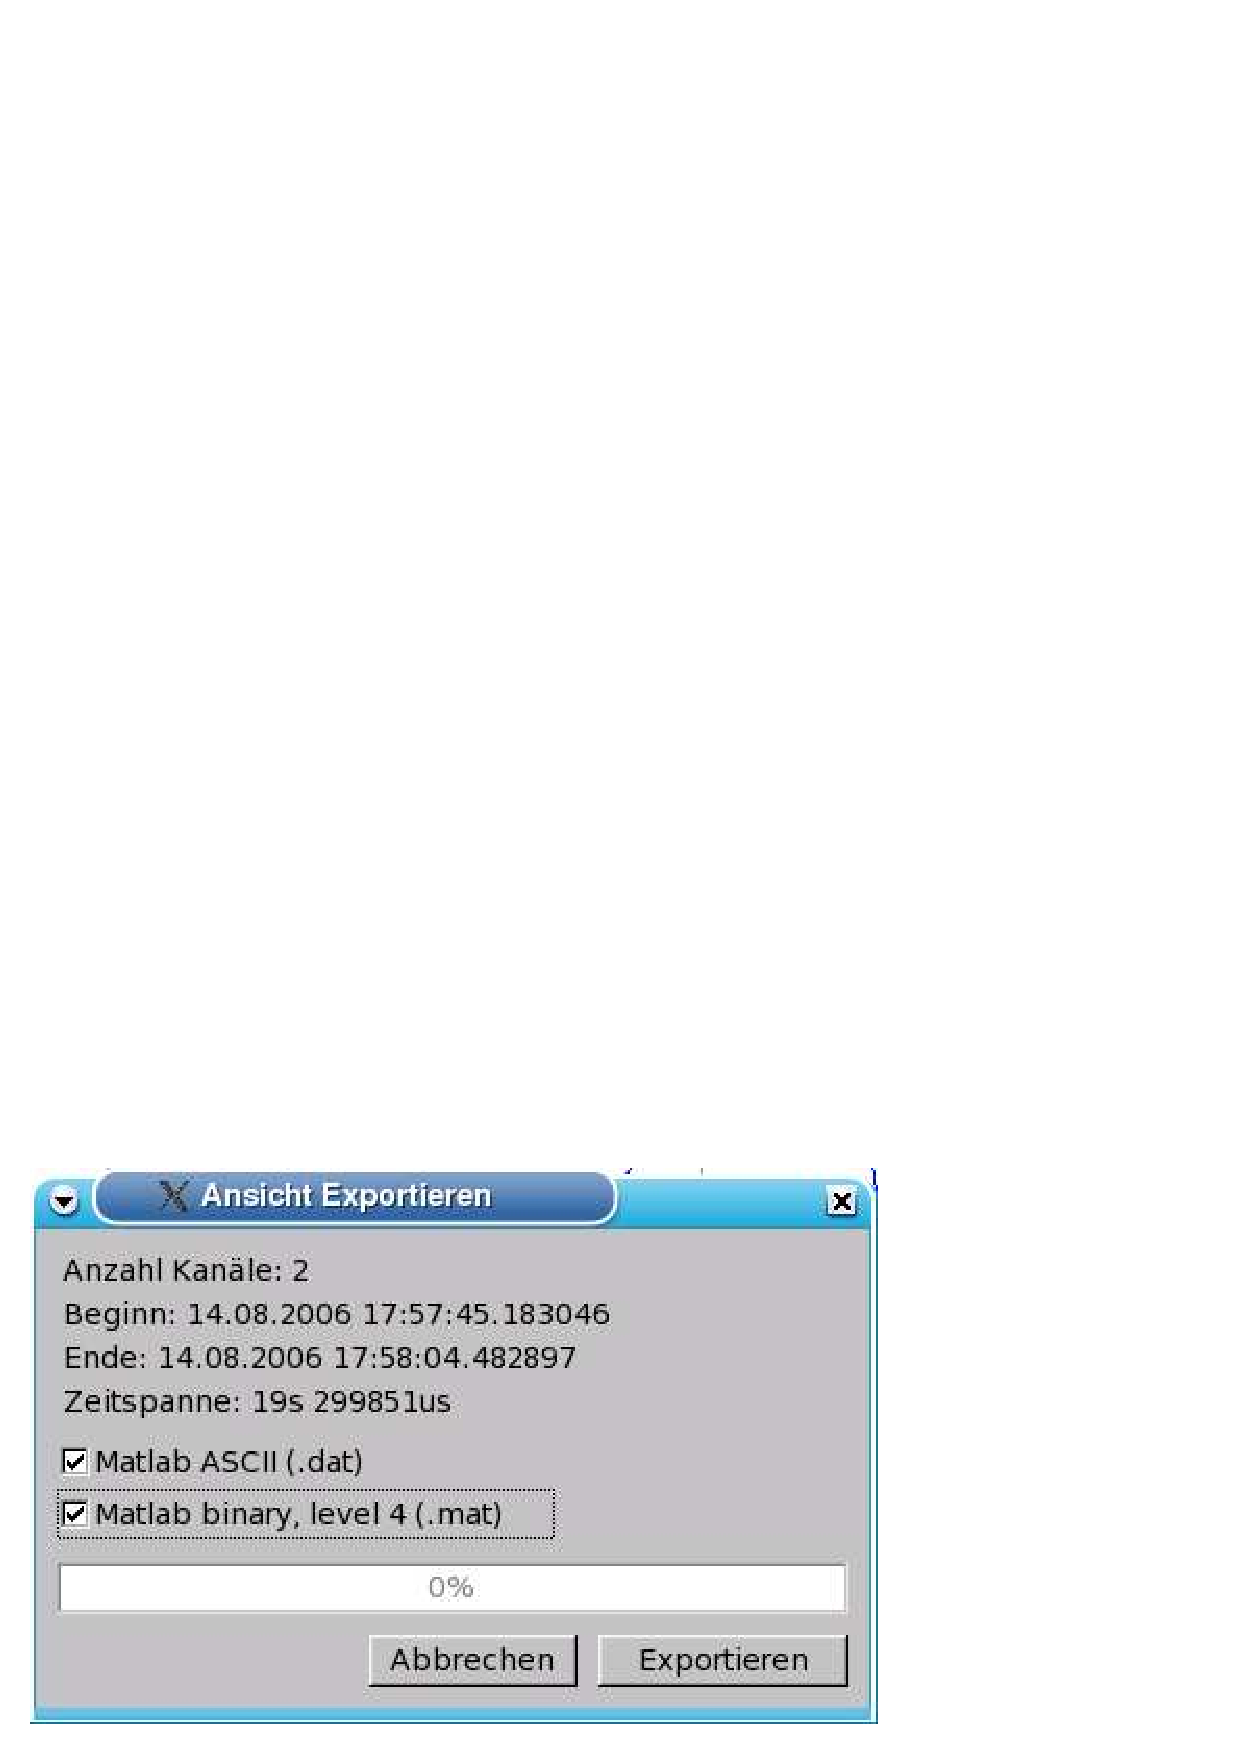
\includegraphics[width=.6\textwidth]{bilder/view_export} \end{center} \caption{Export dialog of DLS View} \label{fig:dls_view_export} \end{figure}

%------------------------------------------------------------------------------

\subsection{Display features}

\begin{itemize}

\item The upper part of the dialog (see \autoref{fig:dls_view_export}) shows
the number of selected channels and the selected time range. The export always
includes the data shown in the currently selected view of the main dialog.

\item The progress bar in the lower part will later show the export progress.

\end{itemize}

%------------------------------------------------------------------------------

\subsection{Interaction features}

\begin{itemize}

\item In the centre part of the dialog (see \autoref{fig:dls_view_export})
check boxes allow selecting the export formats. It is definitely possible to
simultaneously export several formats.

\item A click on the ``Export'' button starts the data export. If the
environment variable \$DLS\_EXPORT\index{\$DLS\_EXPORT} is set, the data will
be written into the corresponding directory. Otherwise, the current directory
will be used. To prevent an overwriting of any data when exporting, a
subdirectory will always be created to accommodate the data files. The name of
this subdirectory is determined by the environment variable
\$DLS\_EXPORT\_FMT\index{\$DLS\_EXPORT\_FMT} , which permits wildcards
according to the conventions of the c function strftime(). See \texttt{man 3
strftime} for a list. If the environment variable has not been set, a default
directory name \textit{dls-export-\%Y-\%m-\%d-\%H-\%M-\%S} is assumed.

\item The ``Cancel'' button interrupts the export and closes the dialog.

\end{itemize}

%------------------------------------------------------------------------------

\chapter{Compression methods} \label{sec:comp} \index{Compression}

The compression of the measured data received from the data source serves to
reduce the required storage space in the file system. It is always done
block-wise (i.\,e. a certain number of data values is always jointly
compressed) with the user being able to adjust the block size in the channel
specifications. A basic distinction is made between lossless and
non lossless compression.

The DLS system supports various compression algorithms. Since most of the algorithms have binary data as output, these will be coded in Base64 before being stored in the data files. Although this results in an expansion of the required storage space by one third, the advantage is that the compressed data will be available in ``printable'' characters and can thus be coded in XML. Therefore, all compression methods of the DLS have the suffix \textit{/Base64}.

The following compression methods are supported by the DLS:

\begin{description}

\item[ZLib/Base64] A simple but efficient compression method offering a
lossless compression. See \autoref{sec:comp_zlib}.

\item[MDCT/ZLib/Base64] An enhanced compression method that processes the data
by a transformation and a quantisation and then only compresses them. See
\autoref{sec:comp_mdct}.

\end{description}


%------------------------------------------------------------------------------

\section{Compression with the ZLib} \label{sec:comp_zlib}

Compression method: ZLib/Base64\\ Compressible data types: all.

The ``ZLib''\index{ZLib} (\url{http://www.gzip.org/zlib}) library provides functions for the lossless compression of data. The dlsd acquisition process uses these functions in the compression method ZLib/Base64. Moreover, the ZLib algorithm is used for support in the subsequent processes to further compress the data already processed.

As the ZLib provides binary data, these will then be stored in all processes coded in Base64.

%------------------------------------------------------------------------------

\section{Compression with the MDCT} \label{sec:comp_mdct} \index{MDCT}

Compression method: MDCT/ZLib/Base64\\ Compressible data types: \textit{TFLT}, \textit{TDBL}

The compression method MDCT (``modified, discrete cosinus
transformation'') of the DLS actually is a hybrid process in which the
data are first transformed with the MDCT, then quantised and finally
bit-wise transposed, in order to render the following compression with
the ZLib more effectively. Here, the intention is to compress the
measured data lossy with limited error.

\subsection{MDCT}

The MDCT is a kind of discrete equivalent to the Fourier
transformation method that transforms a signal into the corresponding
frequency domain which again produces the original signal when overlaid.

While the ``normal'' DCT is based on the principle that $n$ values are
transformed into $n$ coefficients, from which the original signal can then be
completely recovered, the ``modified'' DCT always transforms $n$ values into
$\frac{n}{2}$ coefficients which as such are an incomplete representation of
the original signal. However, as the transformation is performed with 50\%
overlapping, the original signal can be recovered by a re-overlapping of two
successive, re-transformed sequences of coefficients. This method is presented
in \autoref{fig:comp_mdct}.

\begin{figure}[htb] \begin{center} 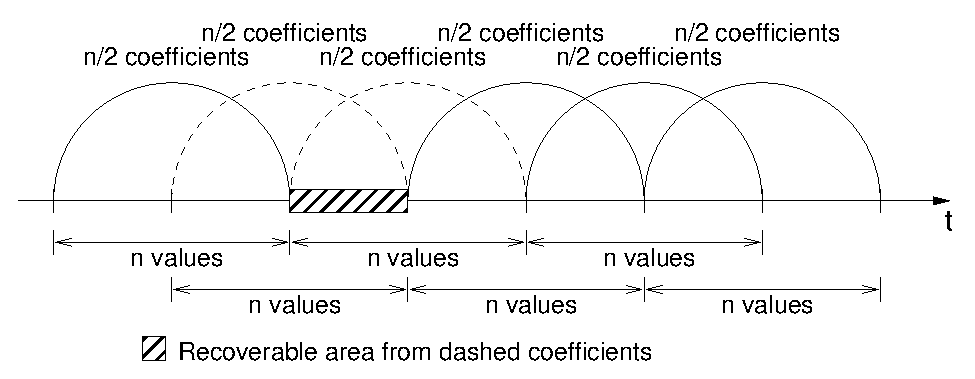
\includegraphics[width=300pt]{bilder/mdct_en} \end{center} \caption{Modified, discrete cosinus transformation} \label{fig:comp_mdct} \end{figure}

This modified DCT is supplemented by the overlaying of the values to be transformed by means of a window function that gives a lower weighting to the values at the margins. It is thus prevented that the different errors on the marginal areas of the single transformations lead to ``artefacts'' and the original signal can be seamlessly recovered.

\subsection{Quantisation}

The coefficients ascertained by the MDCT are subjected to an integer quantisation. Here, a bisection method serves to decide how many bits can minimally be taken for quantisation without the maximum error becoming too large when re-transforming. The quantisation method provides not only the coefficients quantised to $n$ bits but also the floating-point scaling factor required for the recovery of the original coefficient.

As the maximum error cannot exactly be determined for an individual, inverse MDCT, it is estimated by half of the given error. When two sequences of re-transformed coefficients are overlaid for the recovery of the original signal, the given error cannot be exceeded as long as the absolute error in both partial signals does not exceed half of the maximum total error.

Signals from technical processes are frequently most suitable for a transformation by MDCT because in most cases they result from overlaid, harmonic vibrations. This means that the high-frequency portions of the relevant coefficients are often not very pronounced and can largely be adapted by the quantisation. This will lead to a good compressibility later on.

\subsection{Transposition} \label{sec:comp_mdct_trans}

The transposition is needed because the compression method ZLib works byte-wise and in most cases cannot recognise similar bit patterns. So, the individual bits of the quantised coefficients are re-sorted in the memory. For this purpose the coefficients are first of all separated from their algebraic signs. The sign bits are separately stored before the coefficient bits. This is first followed by all \textit{MSB}s (``most significant bits'') of the coefficients and last by all \textit{LSB}s (``least significant bits''). Due to the mostly very small coefficients of the higher-frequencys this results in a lot of zero bytes that can easily be compressed.

Accordingly, a compressed MDCT block consists of the scaling factor of the quantised coefficients (4 byte, or 8 bytes), the quantity $q$ of quantisation bits used (1 byte), $n$ sign bits and finally $q \cdot (n - 1) $ coefficient bits.

\subsection{MDCT via FFT (Fast Fourier Transform)}

Marios Athineos\footnote{marios@ee.columbia.edu,
\url{http://www.ee.columbia.edu/~marios}, Columbia University} has developed a
method to reduce an MDCT via $n$ values to a Fourier transformation\-formation
via $\frac{n}{4}$ values. The DLS employs this method in combination with the
\textit{FFTW3} library (see \autoref{sec:apx_install}) in order to reduce the
computational effort considerably. This library combines efficient algorithms
for the calculation of the Fourier transform with the use of processor
extensions such as MMX or DDE.

%------------------------------------------------------------------------------

\section{Compression through quantisation} \label{sec:comp_quant} \index{quantisation}

Compression method: Quant/ZLib/Base64\\ Compressible data types: \textit{TFLT}, \textit{TDBL}

This loss-afflicted compression method subjects the data values to be compressed to an absolute quantisation, differentiates them and stores them in transposed form. This method prepares the ``raw data'' so that the subsequent compression with the ZLib is even more effective.

\subsection{Quantisation}

During quantisation the individual (floating-point) values are mapped via a scaling factor on a limited interval of the natural numbers. A compression is achieved by trying to keep this interval as small as possible in order to be able to code the quantised values with a few bits. However, this is only done to the extent that the error thus produced remains under a certain limit specified by the user.

\subsection{Differentiation}

In addition, the quantised values are differentiated to have linear signal waveforms become more harmonised in the coding so that the ZLib algorithm can compress the data better. To this end, at the beginning of the compressed data set the (integer) offset is stored and from there onwards always only the difference from value to value is stored.

\subsection{Transposition}

The transposition is done for the same reasons as in the
\textbf{MDCT/ZLib/Base64} method. See \autoref{sec:comp_mdct_trans} in this
respect.

%------------------------------------------------------------------------------

\appendix

\chapter{Installation of the DLS} \label{sec:apx_install} \index{Installation}

\section{System requirements}

The DLS has largely been implemented in the programming language
C++\index{C++}. For compilation and functioning it requires a Linux operating
system\index{Linux}.

The following software must be installed for compilation and at runtime:

\begin{itemize}

\item The \textit{syslogd}\index{syslogd}, which is usually delivered with
every Linux distribution, is used for the recording of the messages being
produced during runtime.

\item For the compilation of the graphical user interfaces DLS
Manager\index{DLS Manager} and DLS View\index{DLS View} it is additionally
necessary to have the GUI library \textit{FLTK}\index{FLTK} in version 1.1
available, which can be downloaded from the FLTK website
\url{http://www.fltk.org}. The library must have been compiled with support
for multithreading\footnote{Unfortunately some Linux distributions only
include a packet without multithreading so that the FLTK library must be
compiled by oneself.} (configure switch \texttt{--enable-threads}).

\item The \textit{ZLib} is required for the compression. This is included in
almost every Linux distribution. In case of need it can be downloaded from
\url{http://www.gzip.org/zlib} and installed.

\item The \textit{FFTW3} library is also required for the compression. This
enables the DLS to compute the Fourier transforms required for the MDCT
compression. The source of supply for the library is
\url{http://www.fftw.org/download.html}.

\item For the DLS Manager and for FLTK you will need the \textit{pthreads}
library.

\end{itemize}

\section{Installation}

After having copied it from the EtherLab\textsuperscript{\textregistered}-CD
or downloading it from the EtherLab\textsuperscript{\textregistered} homepage
\url{http://etherlab.org}, you can unpack the DLS archive:

\begin{lstlisting}
`\$` `\textbf{tar xjf dls-1.0-rXXX.tar.bz2}`
`\$` `\textbf{cd dls-1.0-rXXX.tar.bz2}`
\end{lstlisting}

Now the source code can be configured and compiled with the commands mentioned below. The \texttt{configure} command knows the parameters \texttt{--with-fltk-dir} and \texttt{--with-fftw3-dir} to specify the (deviating) installation directories of the corresponding libraries. The default installation directory of the DLS is \textit{/opt/etherlab}. A different directory can be specified with the parameter \texttt{--prefix}.

\begin{lstlisting}
`\$` `\textbf{./configure}`
`\$` `\textbf{make}`
\end{lstlisting}

A subsequent calling (as \textit{root}) of

\begin{lstlisting}
# `\textbf{make install}`
\end{lstlisting}

will install all necessary executables, scripts and template configuration files.

\section{How to set up DLS as a service}

If the DLS is to be set up as a service, the init script, the sysconfig file and the profile script must be copied into directories that are suitable for distribution. The following commands are suitable for a SUSE Linux distribution but may slightly differ for other distributions:

\begin{lstlisting}
# `\textbf{cd /opt/etherlab}`
# `\textbf{cp etc/init.d/dls /etc/init.d/dls}`
# `\textbf{cp etc/sysconfig/dls /etc/sysconfig/dls}`
# `\textbf{cp etc/profile.d/dls /etc/profile.d/dls}`
# `\textbf{insserv dls}`
\end{lstlisting}

The configuration is made by adjusting the sysconfig file \textit{/etc/sysconfig/dls}. The relevant configuration variables are documented in the file, will later be exported as a environment variable by a profile script and thus be available to all users.

The DLS data directory will automatically be created when the DLS Manager is started. For this purpose either the environment variable \$DLS\_DIR\index{\$DLS\_DIR} must be set or the directory to be initialised must be transferred by means of parameter \texttt{-d}. If the specified directory is not yet a DLS data directory, the user will be asked whether he wishes to initialise it as such.

%------------------------------------------------------------------------------

\chapter{Data types} \label{sec:apx_types}

\autoref{tab:typen} shows all previously supported channel data
types\index{channel!data types} and the respective possible compression methods.

\begin{table}[htb] \centering \caption{Supported channel data types} \label{tab:typen} \vspace{1.5ex} \begin{tabular}[thb]{|l|l|l|} \hline \textbf{Typ} & \textbf{Description} & \textbf{Compression}\\ \hline \textit{TCHAR} & 1 byte integer (with sign) & ZLib/Base64\\ \hline \textit{TUCHAR} & 1 byte integer (without sign) & ZLib/Base64\\ \hline \textit{TINT} & 4 bytes integer (with sign) & ZLib/Base64\\ \hline \textit{TUINT} & 4 bytes integer (without sign) & ZLib/Base64\\ \hline \textit{TLINT} & 4 bytes integer (with sign) & ZLib/Base64\\ \hline \textit{TULINT} & 4 bytes integer (without sign) & ZLib/Base64\\ \hline \textit{TFLT} & 4 bytes floating point & ZLib/Base64,\\ & & MDCT/ZLib/Base64,\\ & & Quant/ZLib/Base64\\ \hline \textit{TDBL} & 8 bytes floating point & ZLib/Base64,\\ & & MDCT/ZLib/Base64,\\ & & Quant/ZLib/Base64\\ \hline \end{tabular} \end{table}

%------------------------------------------------------------------------------

\chapter{PID files} \label{sec:apx_pid}

At several points the DLS system uses so-called \textit{PID} files\index{PID
files}, a mechanism that is to prevent that several processes will run for one
concrete task. A \textit{PID} file contains the \textit{ASCII}-coded process ID
(\textit{PID}) of the currently running process. After each process start it
is therefore determined whether the corresponding file and possibly a process
with the specified PID already exist. If both exist, a new process must not be
started. The process must immediately close itself instead. If no other
instance exists, the newly started process may continue to run and create a
new PID file. Prior to that, an outdated \textit{PID} file (i.\,e. the
specified process no longer exists) can be deleted.

%------------------------------------------------------------------------------

\chapter{Command-line parameters}

%------------------------------------------------------------------------------

\section{dlsd}
\index{dlsd!Command line parameters}

\begin{lstlisting}
dlsd 1.4.0-rc2 revision de0a3e76b9ae
Usage: dlsd [OPTIONS]
  -d <dir>      Set DLS data directory.
  -u <user>     Switch to <user>.
  -n <number>   Set maximal number of open files.
  -k            Do not detach from console.
  -w <seconds>  Wait time before restarting logging
                  process after an error. Default is 30.
  -b            Do not bind to network socket.
  -p <port>     Listen port or service name. Default is 53584.
  -r            Read-only mode (no data logging).
  -h            Show this help.
\end{lstlisting}

%------------------------------------------------------------------------------

\section{Init-Script}
\index{Init-Script!Command line parameters}

(The path may differ depending on the Linux distribution.)

\begin{lstlisting}
USAGE: /etc/init.d/dls {start|stop|restart|status}
\end{lstlisting}

%------------------------------------------------------------------------------

\section{dls\_status}
\index{dls\_status!Command line parameters}

\begin{lstlisting}
Call: dls_status [OPTIONS]
Options:
        -d [directory]     DLS data directory
        -h                 Show this help
\end{lstlisting}

%------------------------------------------------------------------------------

\section{dls\_ctl}
\label{sec:apx_cmd_dlsctl}
\index{DLS Manager!Command line parameters}

The DLS Manager is described in \autoref{sec:manager}.

\begin{lstlisting}
dls_ctl 1.4.0-rc2 revision de0a3e76b9ae
Call: dls_ctl [OPTIONS]
        -d [directory]     DLS data directory
        -u [user]          DLS user
        -h                 Show this help
\end{lstlisting}

%------------------------------------------------------------------------------

\section{dls\_view}
\index{DLS View!Command line parameters}

\begin{lstlisting}
dls_view 1.4.0-rc2 revision de0a3e76b9ae
Call: dls_view [OPTIONS]
        -d [directory]   DLS data directory
        -h               Show this help
\end{lstlisting}

%------------------------------------------------------------------------------

\section{dls}
\label{sec:apx_cmd_dls}
\index{dls (Tool)!Command line parameters}

\begin{lstlisting}
  Usage: dls COMMAND [OPTIONS]
  Commands:
      list - List available chunks.
    export - Export collected data.
      help - Print this help.
  Enter "dls COMMAND -h" for command-specific help.
\end{lstlisting}

%------------------------------------------------------------------------------

\subsection{dls list}

\begin{lstlisting}
  Usage: 1. dls list [OPTIONS]
         2. dls list -j JOB [OPTIONS]

  Description:
         1. Lists all available jobs.
         2. Lists chunks in the specified job.

  Options:
          -d DIR   Specify DLS data directory.
          -j JOB   Specify job ID.
          -h       Print this help.
\end{lstlisting}

%------------------------------------------------------------------------------

\subsection{dls export}

\begin{lstlisting}
dls 1.4.0-rc2 revision de0a3e76b9ae
Usage: dls export [OPTIONS]
Options:
   -d DIR         DLS data directory. Default: $DLS_DIR
   -o DIR         Output directory. Default: $DLS_EXPORT_DIR or "."
   -f NAMEFMT     Naming format for export directory.
                  See strftime(3).
                  Default: $DLS_EXPORT_FMT or "dls-export-%Y-%m-%d-%H-%M-%S"
   -a             Enable ASCII exporter
   -m             Enable MATLAB4 exporter
   -j ID          Job to export (MANDATORY)
   -c CHANNELS    Indices of channels to export (see below).
                  Default: All channels
   -p CHANNEL     Path of one channel to export (see
                  below). This option may appear
                  multiple times. Default: All channels.
   -s TIMESTAMP   Start time (see below). Default: Start of recording
   -e TIMESTAMP   End time (see below). Default: End of recording
   -n DECIMATION  Export every n'th value.
   -g             Export messages.
   -l LANGUAGE    2-character language code for messages.
   -q             Be quiet (no progress bar)
   -h             Print this help
CHANNELS is a comma-separated list of channel indices.
   Use the minus sign to specify ranges.
   Examples: "2,4,9", "1-20", "2,4,13-15,42".
CHANNEL is a signal name, optionally prefixed with
   'FILE:', where FILE is the name of the exported
   channel data file. If FILE is empty, or there is no
   colon found, files are named according to the channel
   indices.
TIMESTAMP is a broken-down time with microsecond resolution:
   YYYY[-MM[-DD[-HH[-MM[-SS[-UUUUUU]]]]]] or
   YYYY[-MM[-SS[ HH[:MM[:SS[.UUUUUU]]]]]].
   Examples: "2006-08", "2005-08-15 13:14:58.896366"
\end{lstlisting}

%------------------------------------------------------------------------------

\section{dls\_quota}
\label{sec:apx_cmd_quota}
\index{dls\_quota!Command line parameters}

\begin{lstlisting}
Call: dls_quota [OPTIONS]
        -d [directory]     DLS data directory
        -i [seconds]       Verification interval (0 = single check)
        -k                 Not a daemon
        -h                 Show this help
\end{lstlisting}

%------------------------------------------------------------------------------

\printindex

\end{document}

%------------------------------------------------------------------------------
